\documentclass[prb,twocolumn]{revtex4-1}
%rmp

\usepackage{graphicx}
\usepackage{color}
\usepackage{latexsym,amsmath}
\usepackage{physics}
%\usepackage{subfig}
\definecolor{linkcolor}{rgb}{0,0,0.65} %hyperlink
\usepackage[pdftex,colorlinks=true, pdfstartview=FitV, linkcolor= linkcolor, citecolor= linkcolor, urlcolor= linkcolor, hyperindex=true,hyperfigures=true]{hyperref} %hyperlink%
\usepackage[backend=biber, sorting=ynt]{biblatex}
%\usepackage{ragged2e} % to justify caption
\addbibresource{bibliography.bib}
\usepackage{tabularx}

\usepackage{fancyhdr}
\pagestyle{fancyplain}% <- use fancyplain instead fancy
\fancyhf{}
\fancyhead[R]{\thepage}
\renewcommand{\headrulewidth}{0pt}

\usepackage{float}
\usepackage{siunitx}




\begin{document}

\title{Nanofabrication, characterization and modelling of gold nanoparticles} 

\author{Alice Pagano}
\author{Alessandra Sabatti}


\date{\today}

\begin{abstract}

The aim of this work is the characterization and modelling of spherical gold nanoparticles synthetized in laboratory by Turkevich method.
At first an absorbance optical measurement was performed on the colloidal solution. The experimental data were modelled using the extinction cross section from the Mie theory, in order to obtain an estimate of the radius of the particles, its density and the refractive index of the medium.
A Grazing-incidence X-ray Diffraction was performed on the nanoparticles deposited on a Si substrate, to get information about the nanoparticle size and its structure.
At last a Scanning Electron Microscope was used to directly measure particle radius and get information about their size distribution.



\end{abstract}

\maketitle


%%%%%%%%%%%%%%%%%%%%%%%%%%%%%%%%%%%%%%
\section{Introduction}

Noble metal nanoparticles show very complex and interesting properties which make them different and more applicable than large size materials \cite{Scaffardi_2006}.
Recently, much attention has been paid towards controlling the shape and size of metal nanostructures because all the magnetic, electrical and optical properties of metal nanostructures are influenced by their shape and size.
Moreover,  gold nanoparticles are of particular interest because of a prominent optical resonance in the visible range.

Colloidal spherical gold nanoparticles can be synthesized by the Turkevich method: gold atoms are decomposed from a gold acid precursor, then they aggregate and growth under controlled constant temperature. The recipe that we follow in this work aim to obtain an average diameter of \(10-20 \text{nm} \).

After synthesis, the optical spectrum of spherical gold nanoparticles is obtained using a Jasco V670 spectrophotometer. The most important information in the absorbance spectrum is the intense absorption line due to the excitation of a surface plasmon resonance. The absorption line is simulated trough the Mie theory in the dipolar approximation, so that we can obtain information on the size of the nanoparticle, its concentration and the refractive index of the medium.

Then, X-rays diffraction is used to compute the average size of spherical gold nanoparticles. We collect the diffraction of X-rays photons, coming from \(\text{Cu}_{k \alpha}\), forming an angle of \(2\theta\) with respect to the incoming beam. In particular, a grazing incidence is used to obtain information only from the sample surface.

Finally, the particle size and shape is derived from scanning electron microscopy images, obtaining the statistical size distribution of the system. 



\section{Chemical synthesis}
The Turkevich method is used to produce size-defined spherical gold nanoparticles trough chemical reduction \cite{article}. The following protocol aims to obtain nanoparticles of about \(10-20 \text{nm} \) of diameters:

\begin{itemize}
\item pour in the beaker \(9.5\text{mL}\) of gold hydroclorate solution (\( \text{HAuCl}_4\));
\item rise the temperature of the gold solution filled with water up to \(100^\circ\). Then, activate the stirrer to have a homogeneous distribution of temperature and concentration.
\item Heat the sodium citrate solution (\( \text{Na}_5 \text{C}_6 \text{H}_5 \text{O}_7 \)) up to  \(100^\circ\).

\item When both solutions are at  \(100^\circ\), add  \(0.5\text{mL}\) of the \(\text{Na}\) reducing agent into the baker. It decomposes the precursor by redox reduction, so that gold atoms are reduced to metallic gold. The citrate concentration is chosen to achieve particles sizes of \(10-20 \text{nm} \) of diameters, in a way to prevent the formation of big structures.

\item Then, wait 15 minutes with the stirrer on and at \(100^\circ\).
\end{itemize}



\section{Optical spectroscopy}

\subsection{Method}
Once the nanoparticles are synthesized, we want to acquire the absorbance spectrum and verify the presence of the localized surface plasmon resonance. We acquire an optical spectrum by using a JASCO double beam spectrophotometer. It shines light in a continuous spectrum ranging from $300$ nm up to $2700$ nm. 

In order to make a spectral measurement, a single-wavelength at a time is selected by a monocromator and then it incides on the sample; for this particular measurements we select a resolution of $1$ nm. The same thing is done by a second beam, which provides a base-line. Then the transmitted intensity is measured for each wavelength. This data is recast by the software into absorbance data, which is related with the trasmittance $T$ by the Lambert-Beer formula:
\begin{equation}
    A \equiv \log_{10} \frac{1}{T}
\end{equation}
At first, we measure the spectrum for the medium in which nanoparticles are immersed, which is water and tetrachloroauric acid, in order to acknowledge the spectral features of the medium. Then, we measure the gold nanoparticle solution spectrum. Both experimental spectra are illustrated in Fig.\ref{fig:exp_spectra}.
As expected, we see a resonant peak at about $\lambda = 529$ nm.

\begin{figure}[!t]
    \begin{minipage}[l]{1.0\columnwidth}
    \centering
    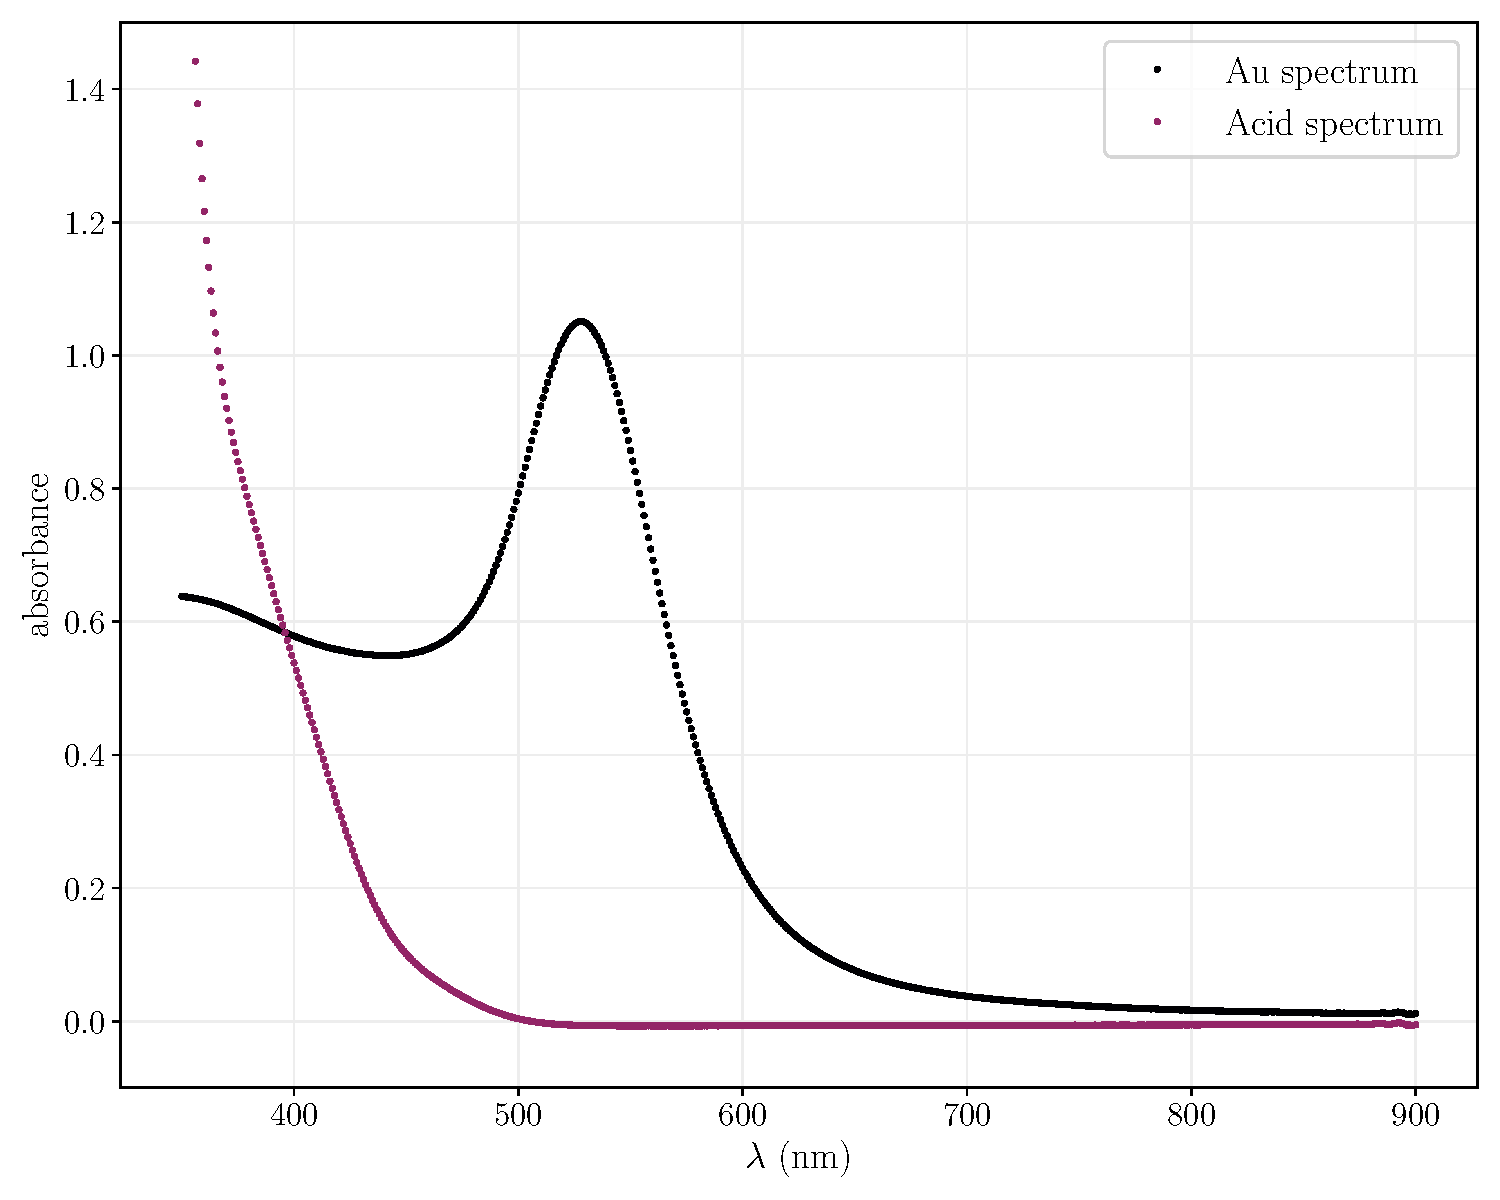
\includegraphics[width=0.9\textwidth]{images/os/exp_data.pdf}
    \caption{In black is represented the Gold nanoparticle experimental spectrum, while in violet the acid spectrum.}
    \label{fig:exp_spectra}
    \end{minipage}
\end{figure}
We can model this spectrum using the extinction cross section coming from Mie Theory in dipolar approximation, upon some assumptions:
\begin{itemize}
    \item we assume that the system is monodispersed with respect to the particle radius;
    \item the nanoparticle dimension is much smaller than the injected wavelengths: $R \ll \lambda$;
    \item we assume a regime of independent nanoparticles: particles are not affected by each other scattering field;
    \item the medium dielectric function is real: $\epsilon_m(\omega) \in R$;
    \item the nanoparticle dielectric function is size-dependent according to the following equation:
    \begin{small}
    \begin{equation}
    \begin{split}
       \epsilon(\omega,R) & = \epsilon(\omega,\infty) + \omega_P^2 \qty(\frac{1}{\omega^2+\Gamma_{\infty}^2}-\frac{1}{\omega^2+ \Gamma(R)^2)}) \\ 
     & -i\frac{\omega_P^2}{\omega} \qty(\frac{\Gamma_{\infty}}{\omega^2+\Gamma_{\infty}^2}-\frac{\Gamma(R)}{\omega^2+ \Gamma(R)^2)})
      \end{split} 
    \end{equation}
    \end{small}
    \noindent where $\omega_P$ is the plasmon frequency of bulk gold, $\Gamma(R) = \Gamma_{\infty} + \pi v_{Fermi}/4R$ is the size-dependent electrons relaxation frequency according to Drude model and $\Gamma_{\infty}$ is the relaxation frequency in bulk gold.
\end{itemize}
 The constant bulk values for Gold are reported in Tab. \ref{tab:constant_bulk}.
 
    \begin{table}[H]
    \centering
    \begin{tabular*}{\columnwidth}{@{\extracolsep{\fill}}ccc}
    \toprule
    \( \pmb{ \omega_P } \) \cite{PhysRevB.6.4370} & \(\pmb{ \Gamma_{\infty} } \) \cite{PhysRevB.6.4370} & \( \pmb{ v_{Fermi} }  \) \cite{ashcroft2011solid} \\
    \colrule
    \(1.37\times 10^{16} \) Hz & \(1.08 \times 10^{14} \) Hz & \(1.4     \times 10^{6}\) m/s \\	   
    \botrule
    \end{tabular*}
    \caption{Bulk Gold constant values at room temperature.}
    \label{tab:constant_bulk}
    \end{table}
    
    
The size correction of the dielectric function is illustrated in Fig.\ref{fig:size_correction} for different values of the radius.
\begin{figure}[H]
    \begin{minipage}[l]{1.0\columnwidth}
    \centering
    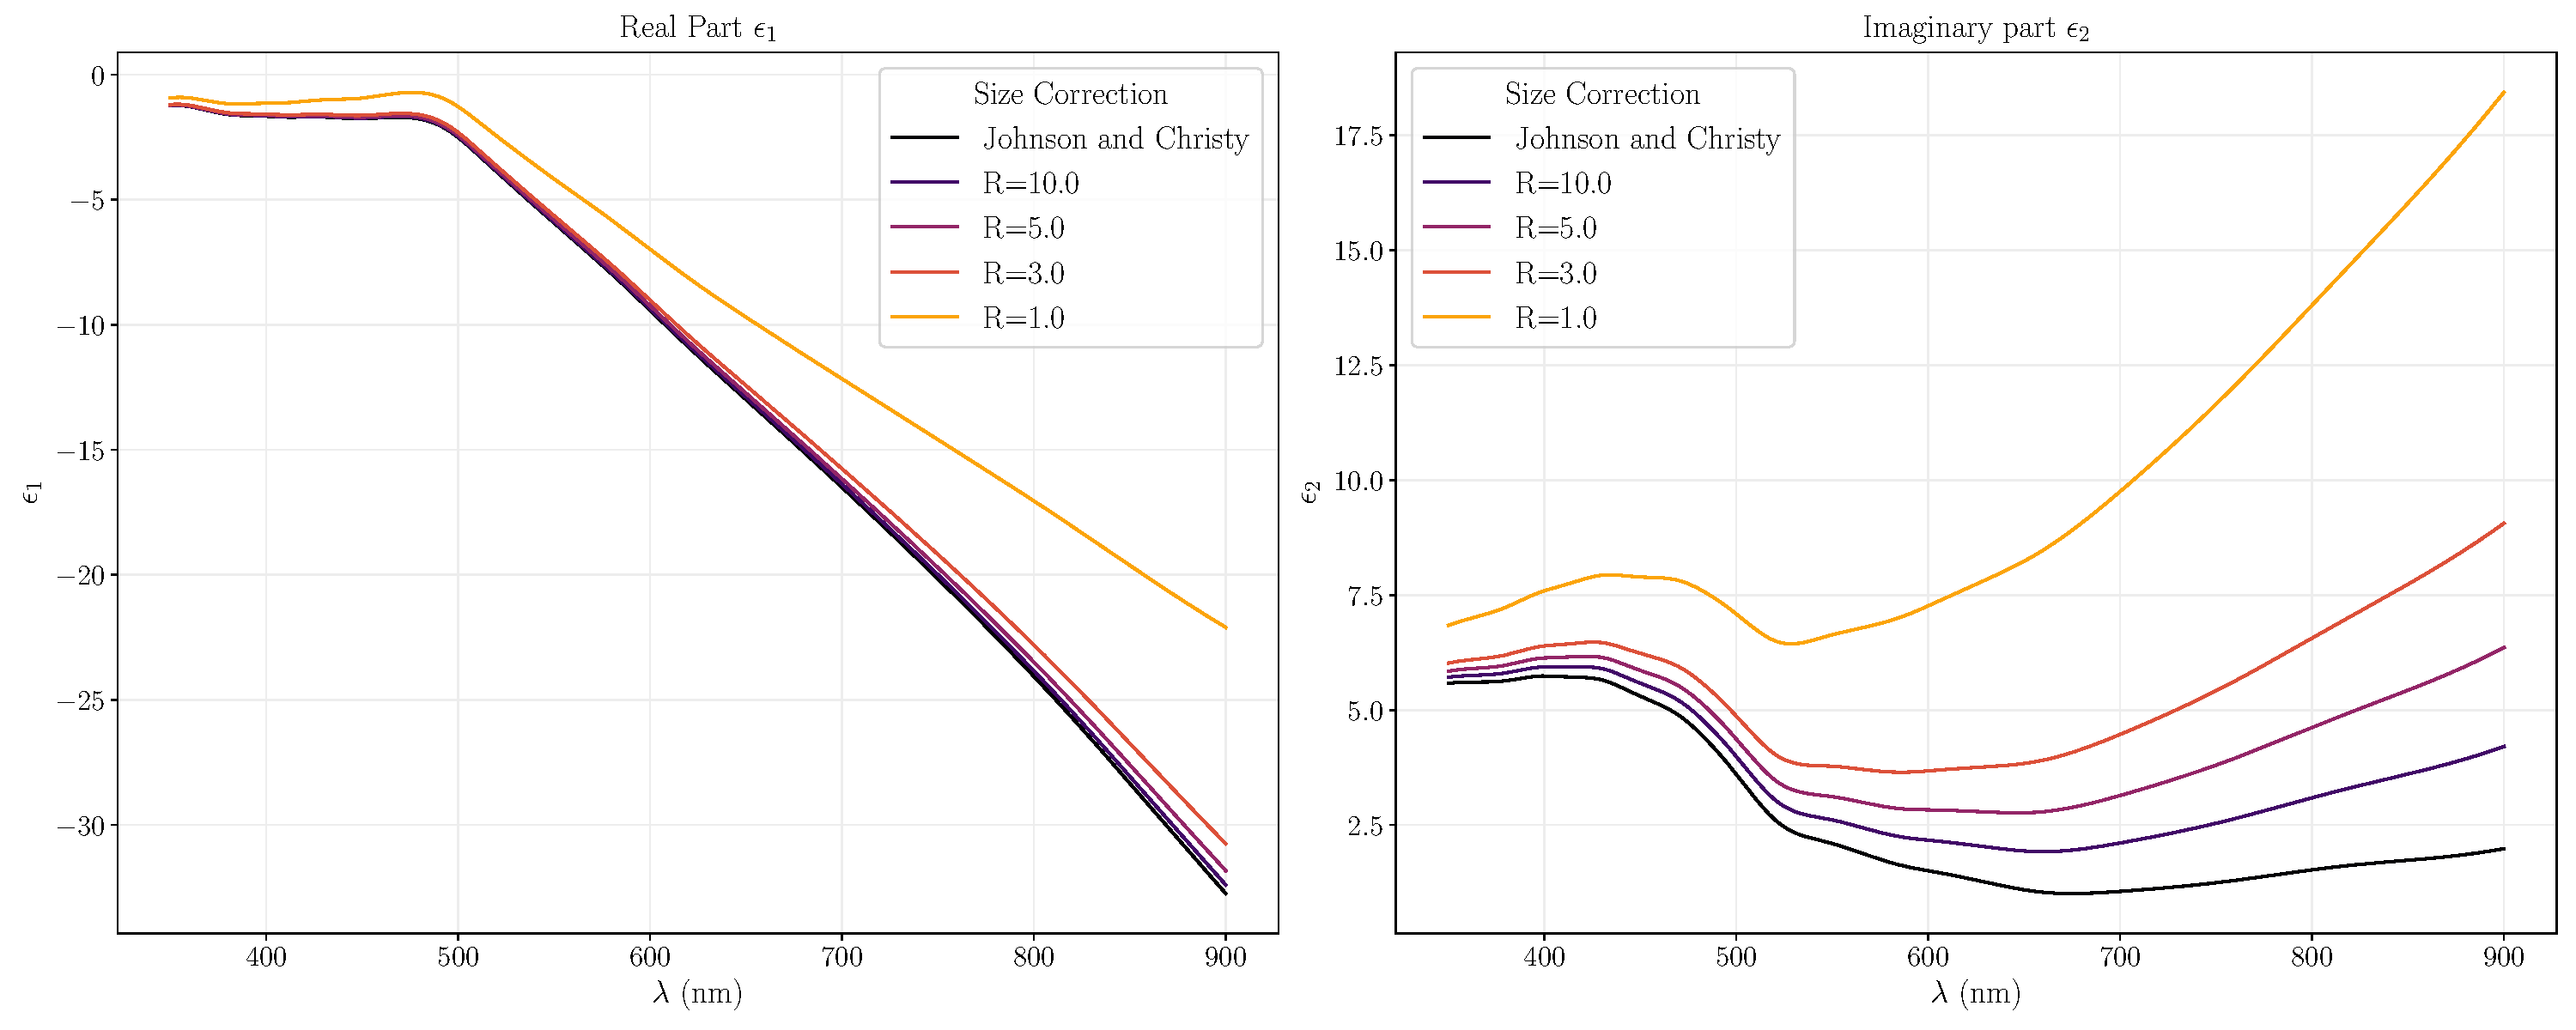
\includegraphics[width=0.95\textwidth]{images/os/size_correction.pdf}
    \caption{Size correction of the dielectric function for different values of the radius. Johnson and Christhy label refers to non size corrected dielectric values.}
    \label{fig:size_correction}
    \end{minipage}
\end{figure}


The absorbance expression obtained with these assumptions is the following:
\begin{equation}
A = C \rho \omega \epsilon_m^{3/2} R^3 \frac{\epsilon_2  }{(\epsilon_1 + 2\epsilon_m)^2+(\epsilon_2 )^2}
\label{eq:absorbance}
\end{equation}
with $C = log_{10}(e)z\frac{9}{c}\frac{4\pi}{3}$.

We notice that a model with a size-independent value for gold dielectric constant $\epsilon(\omega)$ is useless, because the quation \ref{eq:absorbance} contains the product of $R$ and $\rho$, so the parameters cannot be computed independently. Hence, we directly use a size-dependent equation, considering $\varepsilon_1(\omega,R)$ and $\varepsilon_2(\omega,R)$.

In order to simulate the experimental absorbance, we vary the values of the three parameters R, $\rho$ and $\epsilon_m$ inside suitable ranges as follow:
\begin{itemize}
    \item at first, we vary R and $\rho$ keeping $\epsilon_m$ constant. Thus, we obtain the fit for the couple $(R,\rho)$; 
    \item then, we find the values minimizing the $\chi^2$ function, which is defined as follow:
        \begin{equation}
        \chi^2 = \qty(\frac{A_{exp}-A_{sim}}{\sigma_{A_{exp}}})^2
        \end{equation}
        where \( {\sigma_{A_{exp}} = 1/A_{exp} \) is the error associated to the experimental absorbance. We choose this value for the error in order to give a different weight to the spectrum values and eventually obtain a better agreement between data and simulation;
   \item we fix the value of $\rho^*$ obtained from previous simulation and vary $R$ and $\epsilon_m$, obtaining the fit for the couple $(R,\epsilon_m)$. Again, we compute the minimum $\chi^2$ for these parameters;
   \item the value of $\rho^*$ from the first minimization and the values of $R^*$ and $\epsilon_m^*$ from the second minimization are the final parameters;
\end{itemize}
We compute the filling fraction $f=\rho V$ in order to verify the assumption of non-independent particles.

\begin{figure*}[t!]
    \centering 
    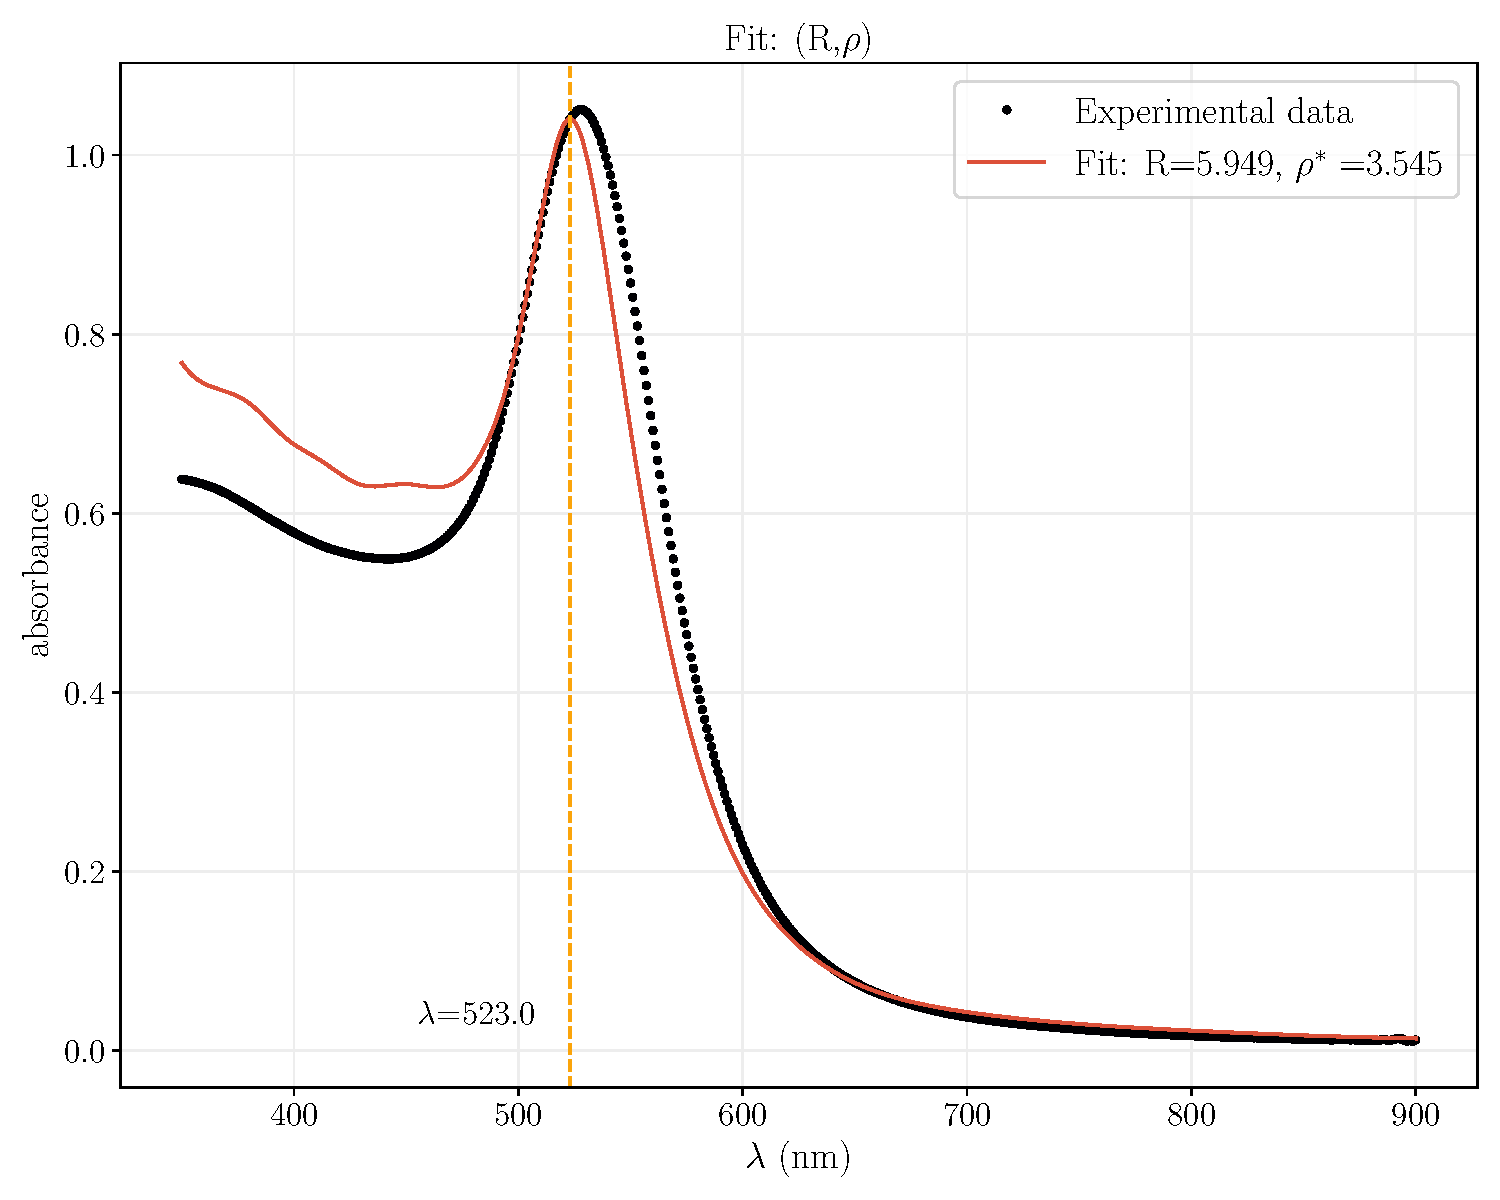
\includegraphics[width=0.49\textwidth]{images/os/1_fit.pdf}
    \hskip 1mm
   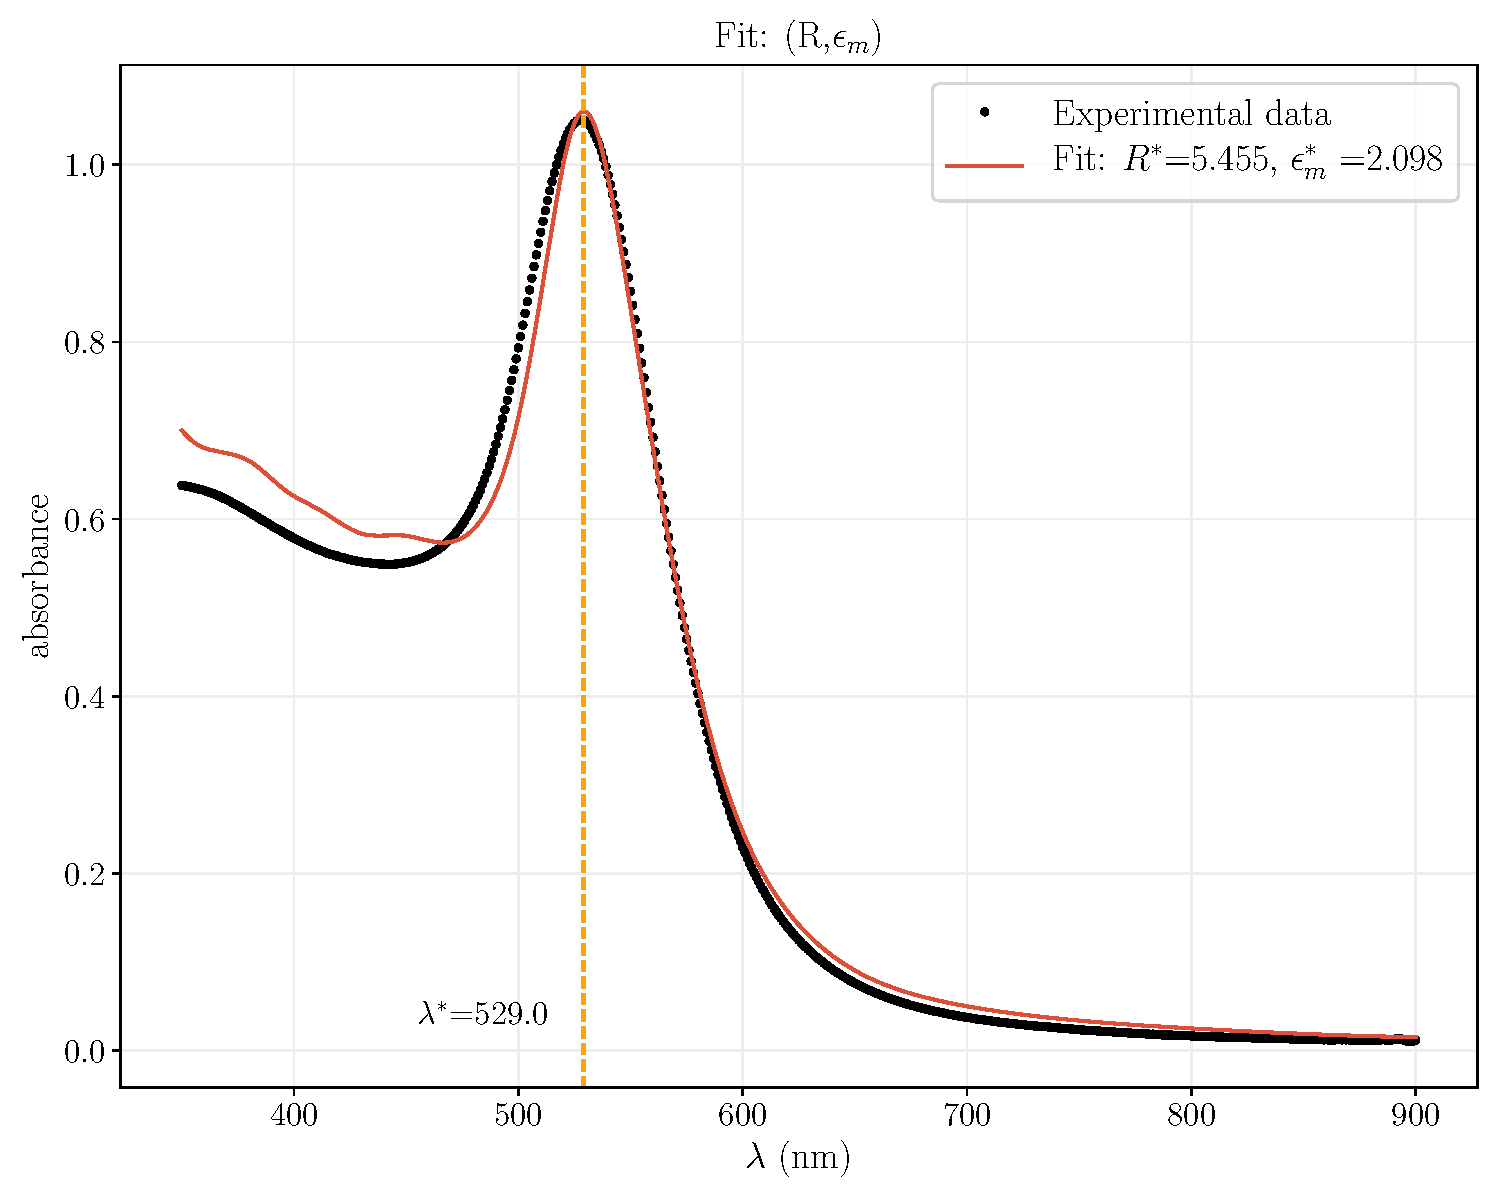
\includegraphics[width=0.49\textwidth]{images/os/2_fit.pdf}
    \\
    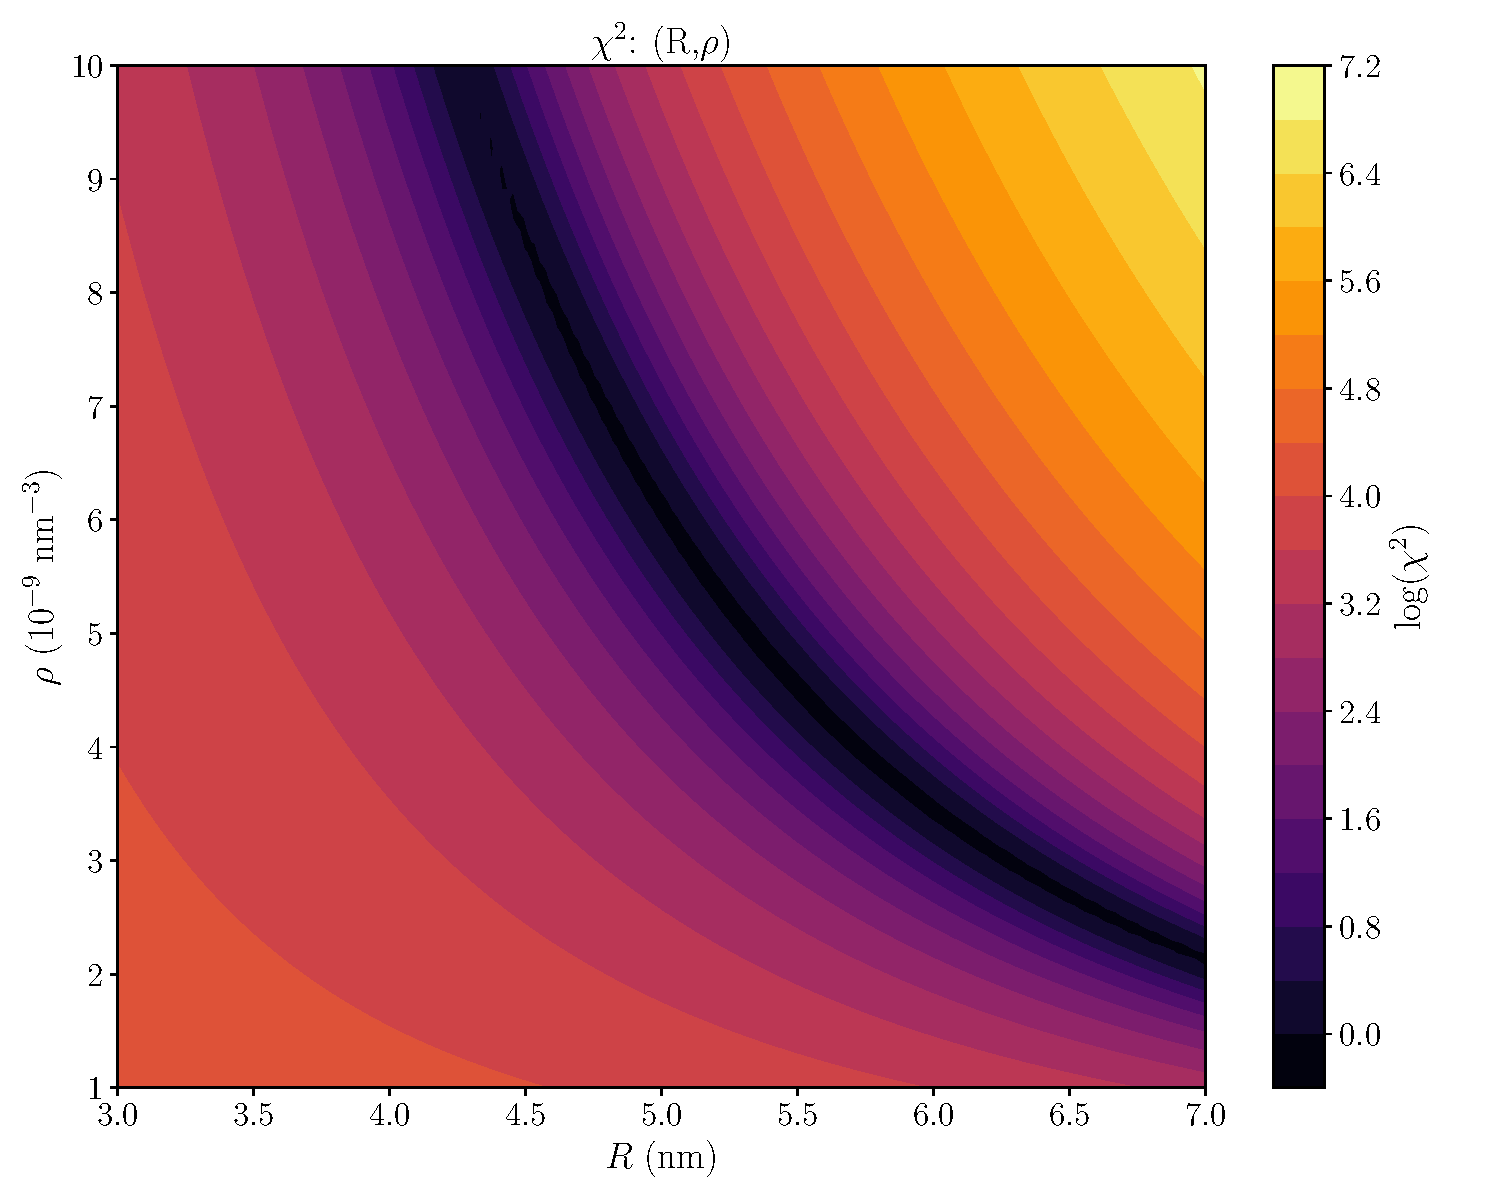
\includegraphics[width=0.49\textwidth]{images/os/1_chisquare.pdf}
   \hskip 1mm
   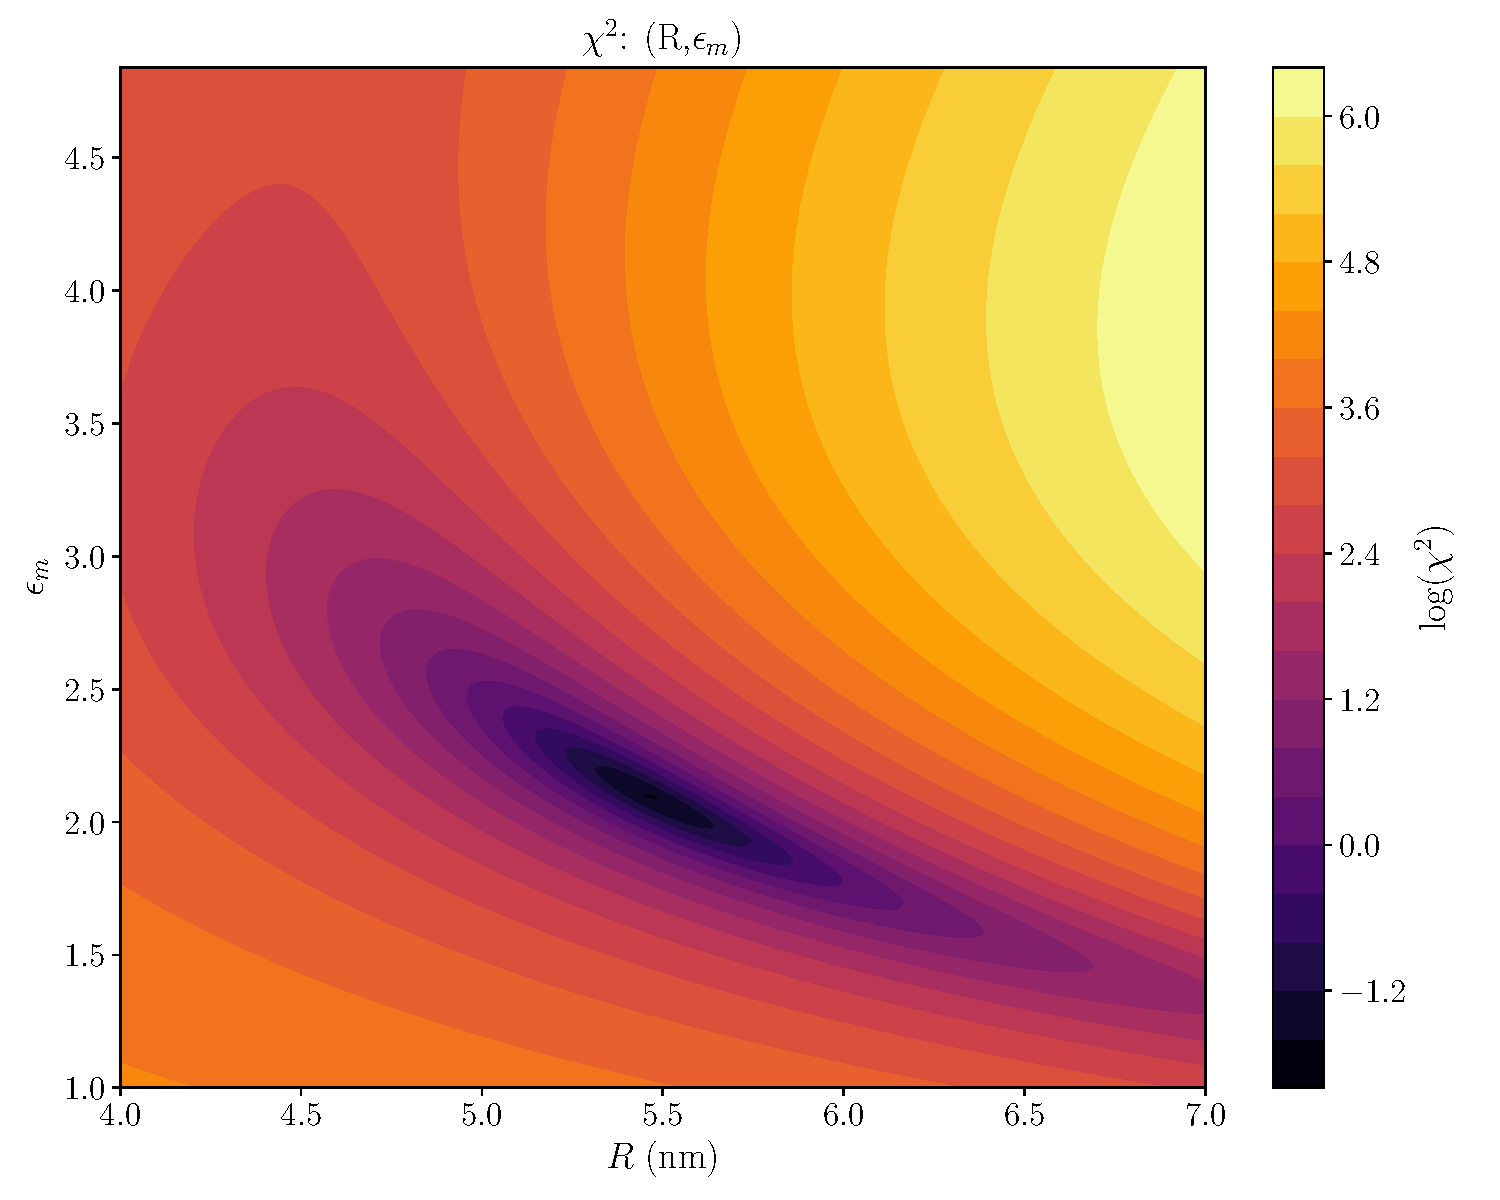
\includegraphics[width=0.49\textwidth]{images/os/2_chisquare.pdf}
    \caption{Mie theory. \textbf{Top}: on the left is represented the simulated spectrum obtained by varying the parameters $(R,\rho)$, while on the right the one obtained varying $(R,\epsilon_m)$. \textbf{Bottom}: on the left we have the $\chi^2$ map for $(R,\rho)$, on the right the one for $(R,\epsilon_m)$. }
    \label{fig:optical_results}
\end{figure*}


To obtain a better agreement with the experiment, we make a further correction disregarding the assumption of size-monodispersed system. We assume a log-normal distribution for the nanoparticle size:
\begin{equation}
f(r;A,\mu,\sigma) = \frac{A}{r\sigma\sqrt{2\pi}}\exp(-\frac{(\ln(r)-\mu)^2}{2\sigma^2})
\label{eqn:log_normal}
\end{equation}
The mean value of the distribution is $\exp(\mu+\sigma^2/2)$, so we choose $\mu$ such that the mean corresponds to the $R$ we want to simulate. For parameter $\sigma$ we choose a value which represents a reasonable dispersion. 
Then, we  repeat the minimum $\chi^2$ analysis, considering as $R$ the mean of the log-normal distribution. 



\subsection{Results}


At first, we simulate the spectrum for the couple $(R,\rho)$, fixing as dielectric constant for the medium the water one, $\epsilon_m = 1.33^2$. As we expect an average radius between $5$ and $10$ nm, we vary $R$ inside the range $[3:15]$ nm, whereas for $\rho$, we make a preliminar trial in order to find its magnitude order. A suitable range obtained is $[1,10]\cdot 10^{-9} \text{nm}^{-3}$. The simulated spectrum obtained from this first fit has not a good agreement with the experimental one, as illustrated in Fig.\ref{fig:optical_results}. \\
Then, we make the fit for $(R,\epsilon_m)$ couple. We vary $R$ in the same range as before, while for $\epsilon_m$ we choose $[1.5:2.5]$.
From this second fit, we get a value for $\epsilon_m^*$ quite different than the one we fixed in the $(R,\rho)$ fit. This improves the agreement with the experimental spectrum (Fig.\ref{fig:optical_results}), even if there is still a poor fit quality for low $\lambda$. This may be due to the non-absorbing medium approximation: as shown in Fig.\ref{fig:exp_spectra}, the absorbance for low wavelengths is quite high.

The obtained values are:
\begin{equation*}
    R^* = 5.455  \text{nm}, \quad \rho^* = 3.545 \cdot 10^{-9} \text{nm}^3 , \quad \epsilon_m^* = 2.098
\end{equation*}

In order to verify the stability of our parameters, we plot the $\chi^2$ map as a function of the two couples of parameters \( (R,\rho) \) and \( (R,\epsilon_m) \). The two maps are illustrated on the bottom of Fig.\ref{fig:optical_results}.

From the \( (R,\rho) \) plot, we observe that we do not get an isolated minimum for $\chi^2$, but there is an elongated region with low $\chi^2$. This may be due to the correlation between $R$ and $\rho$ in the absorbance formula. In the \( (R,\epsilon_m) \) plot of $\chi^2$, we can see that the stability region is more sharp, so the value for $\epsilon_m$ is probably more precise. We try to associate to these estimates an error coherent with these $\chi^2$ maps, but, especially for the density, the uncertainty is very high; giving an estimate with such a big error is probably meaningless.

To summarize, from this analysis, the best values for the three parameters $R$, $\rho$, $\epsilon_m$ are:
\begin{equation*}
    R^* = (5\pm 1)  \text{nm}, \quad \rho^* = (4 \pm 2) \cdot 10^{-9} \text{nm}^3 , \quad \epsilon_m^* = 2.1 \pm 0.1
\end{equation*}

Since the filling fraction results $f=2.4 \times 10^{-6}$, the assumption of independent particles holds. Indeed, the distance between particles is so high that single scattering events can be considered. We can also justify the dipolar approximation, since the particle radius is less then 20 times smaller than the wavelength.

Moreover, the best value for the position of the peak is $\lambda^* = 529\, \text{nm}$ which agrees with the Mie theory. 

Eventually, we repeat the analysis by assuming a log-normal size distribution. In Fig.\ref{fig:size_distribution} we report the histogram for the log-normal centered in the average radius $R^*=5.455$, found by the previous analysis, and with $\sigma=0.1$. However, the agreement of the simulated spectrum obtained with the size-distribution does not improve with respect the one of a monodispersed system.



\begin{figure}[htp]
    \begin{minipage}[l]{1.0\columnwidth}
    \centering
    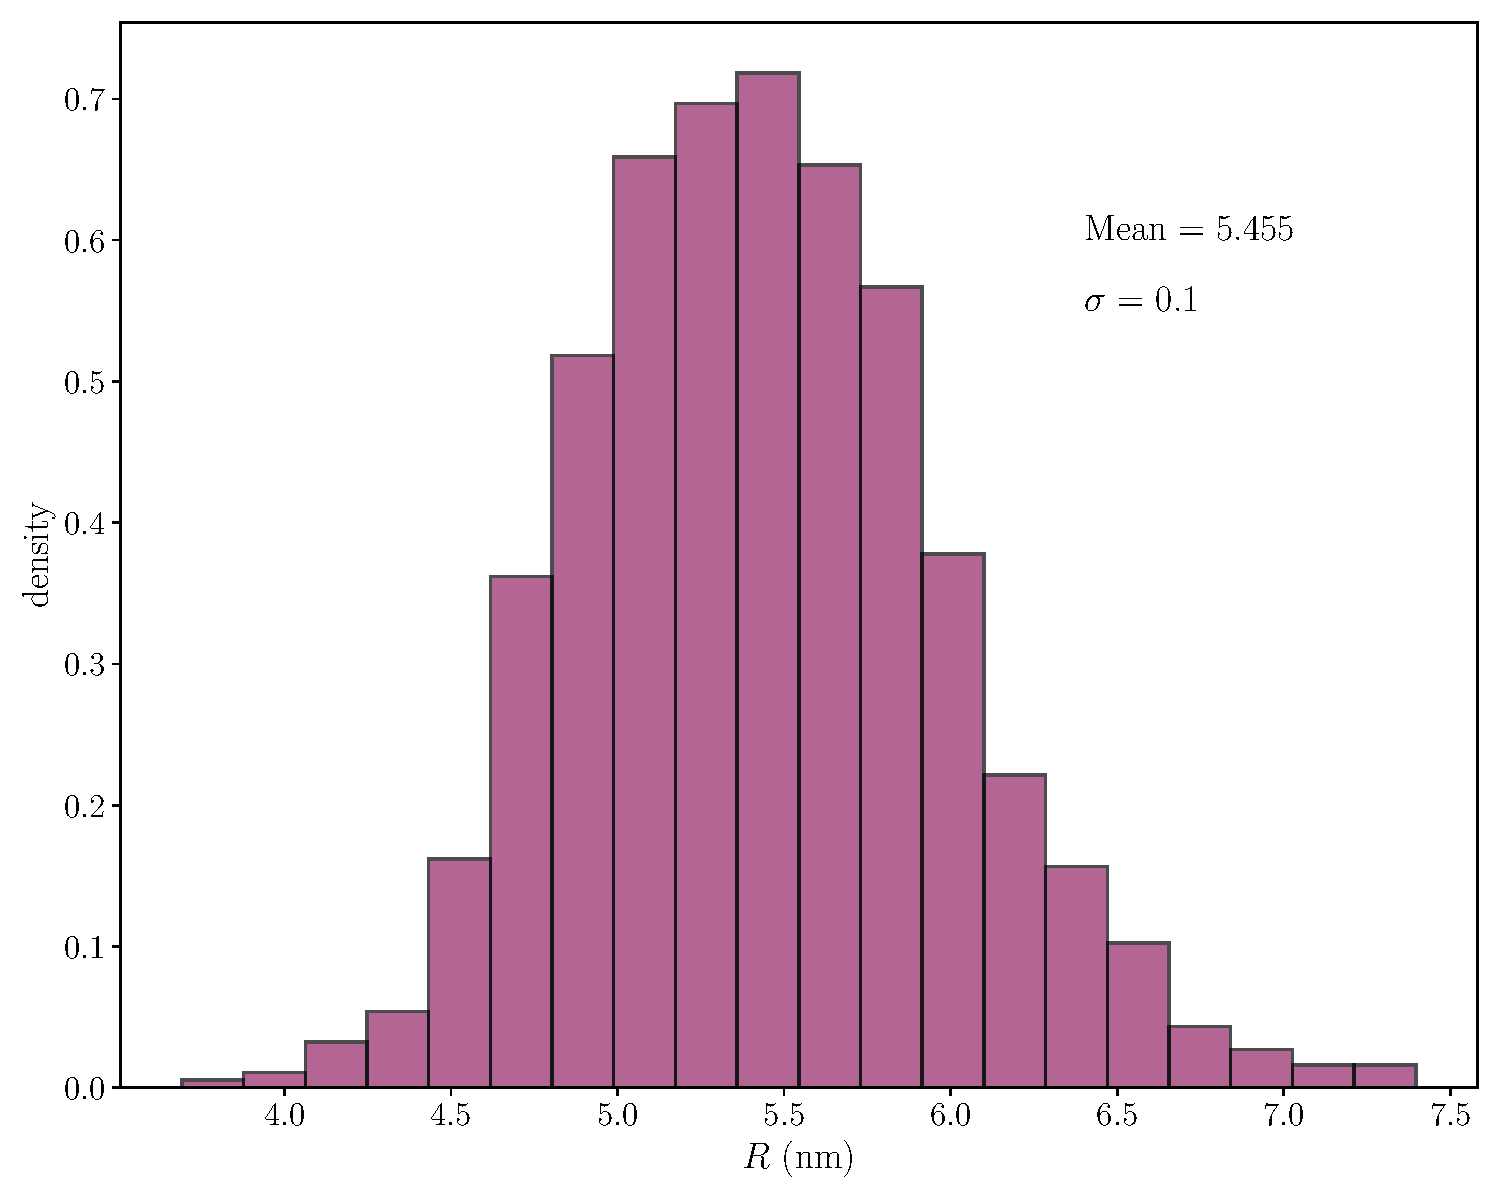
\includegraphics[width=0.9\textwidth]{images/os/size_distribution.pdf}
    \caption{Log-normal size distribution centered around the average value of the radius of $R^*=5.455$ with $\sigma=0.1$.}
    \label{fig:size_distribution}
    \end{minipage}
\end{figure}








\section{X-ray Scattering Analysis}

\subsection{Method}
Before proceeding with X-rays diffraction measurement acquisition, we need to immobilize the gold nanoparticles on a rigid substrate. Hence, we use APTES (3-Aminopropyl) triethoxysilane to fix the nanoparticles in a substrate of monocristalline sample of silica. 

X-rays diffraction is used to obtain information on the structure of a given compound. We consider X-rays photons coming from a \(\text{Cu}\) source of \(\lambda=0.154 \text{nm}\). 
We collect the intensity emerging from the scattering of the incident beam with the sample of gold nanoparticles, forming an angle \(2\theta\) with respect to the incoming beam. In particular, we scan the sample in a horizontal plane using the X-ray diffractometer (X'Pert PRO). Moreover, in order to obtain information only from the surface of the sample and to improve the signal-to-noise ratio, we keep the incidence angle fixed at a grazing incidence of \(\omega=0.6^\circ\) with respect to the horizontal plane. 



In Fig.\ref{fig:scattering_intensity} it is showed the experimental scattering intensity of gold nanoparticles. We assign the Miller indexes to each peak in the spectrum assuming f.c.c.  structure for gold. 
Note that we disregard the peaks in the range of \(50^\circ-60^\circ \) because their origin is due to the interaction with the silycon substrate.

\begin{figure}[htp]
    \begin{minipage}[l]{0.9\columnwidth}
        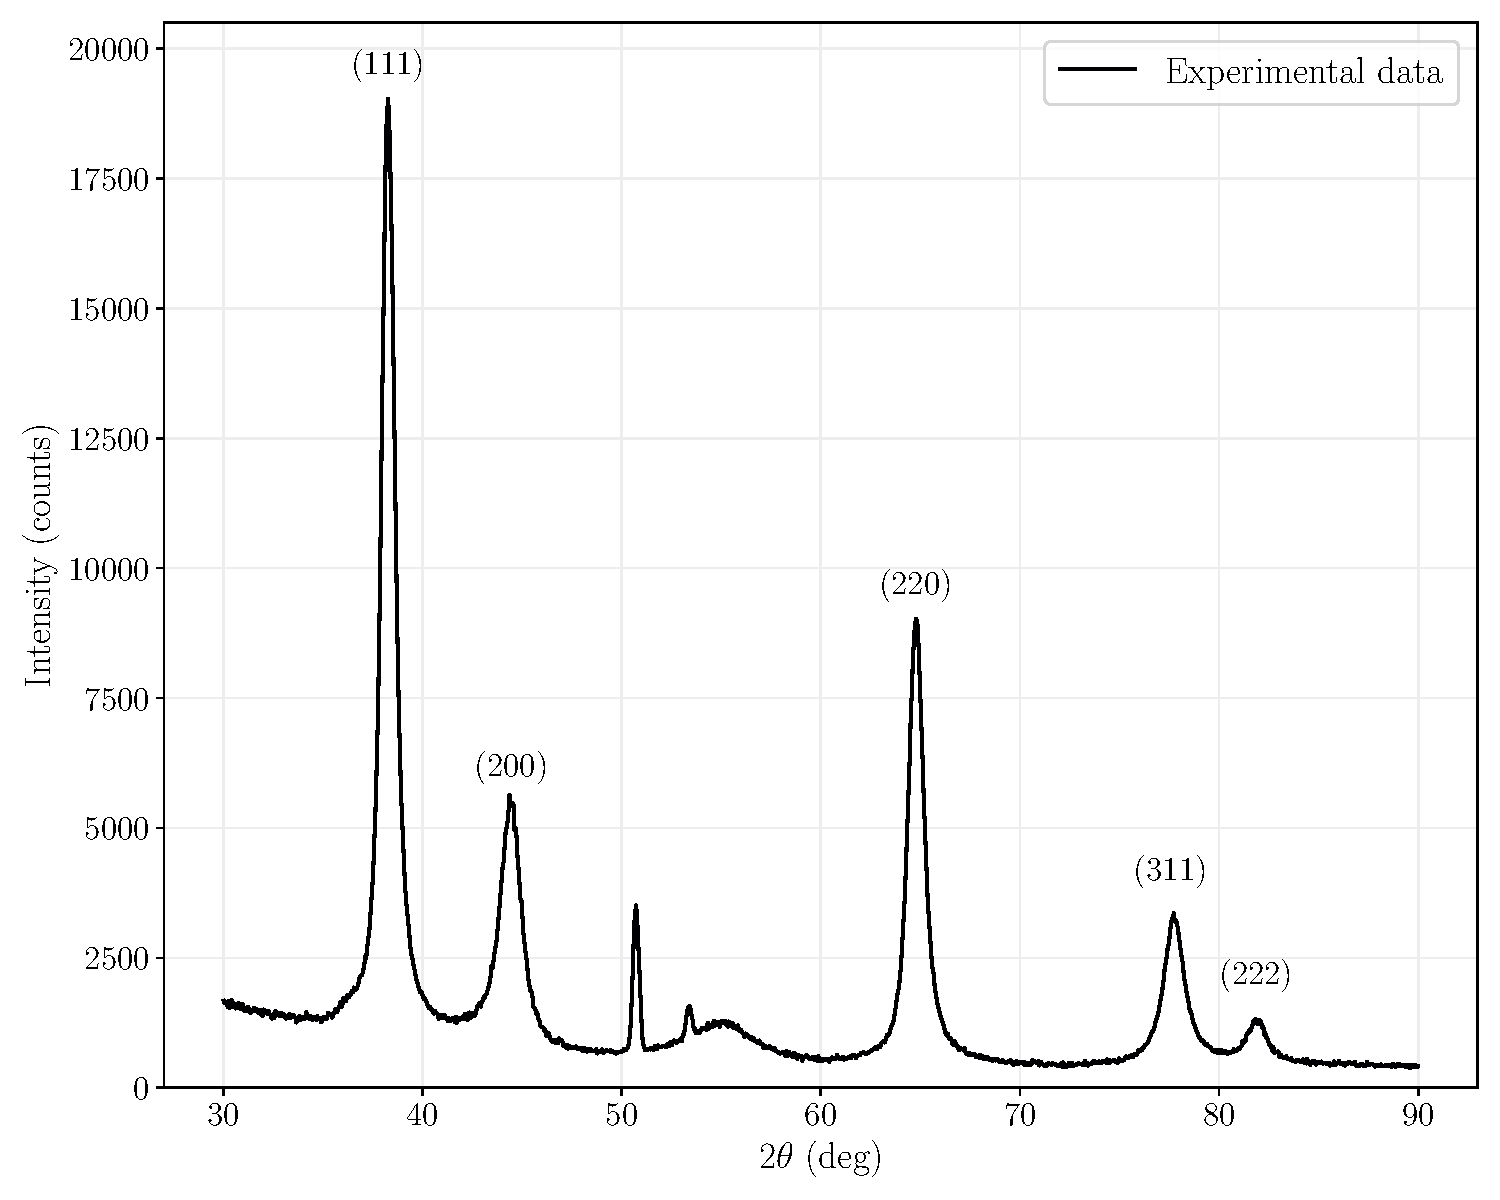
\includegraphics[width=1.0\textwidth]{images/xrd/scattering_intensity.pdf}
        \caption{Experimental scattering intensity of gold nanoparticles as a function of the scattering angle \(2 \theta\). The peaks corresponding to the different lattice planes in f.c.c. gold are labeled.}
        \label{fig:scattering_intensity}
    \end{minipage}
\end{figure}




\begin{figure*}[t!]
    \centering 
    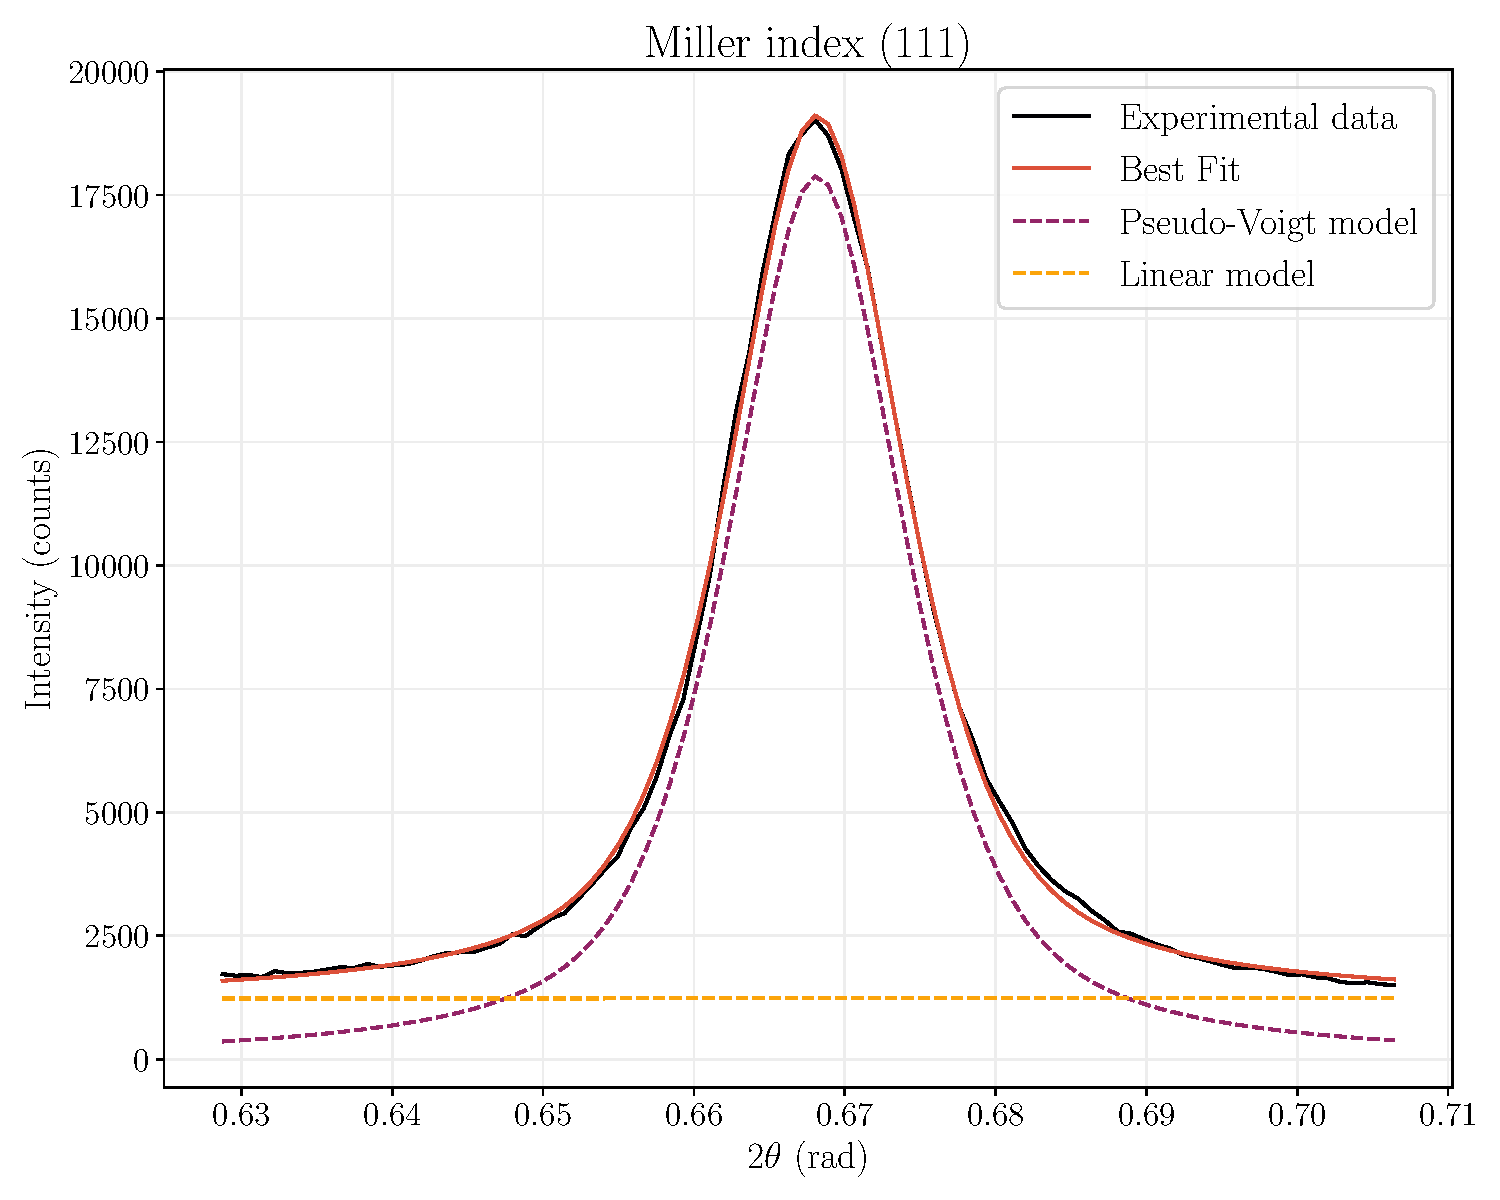
\includegraphics[width=0.3\textwidth]{images/xrd/1_peak.pdf}
    \hskip 0.01mm
    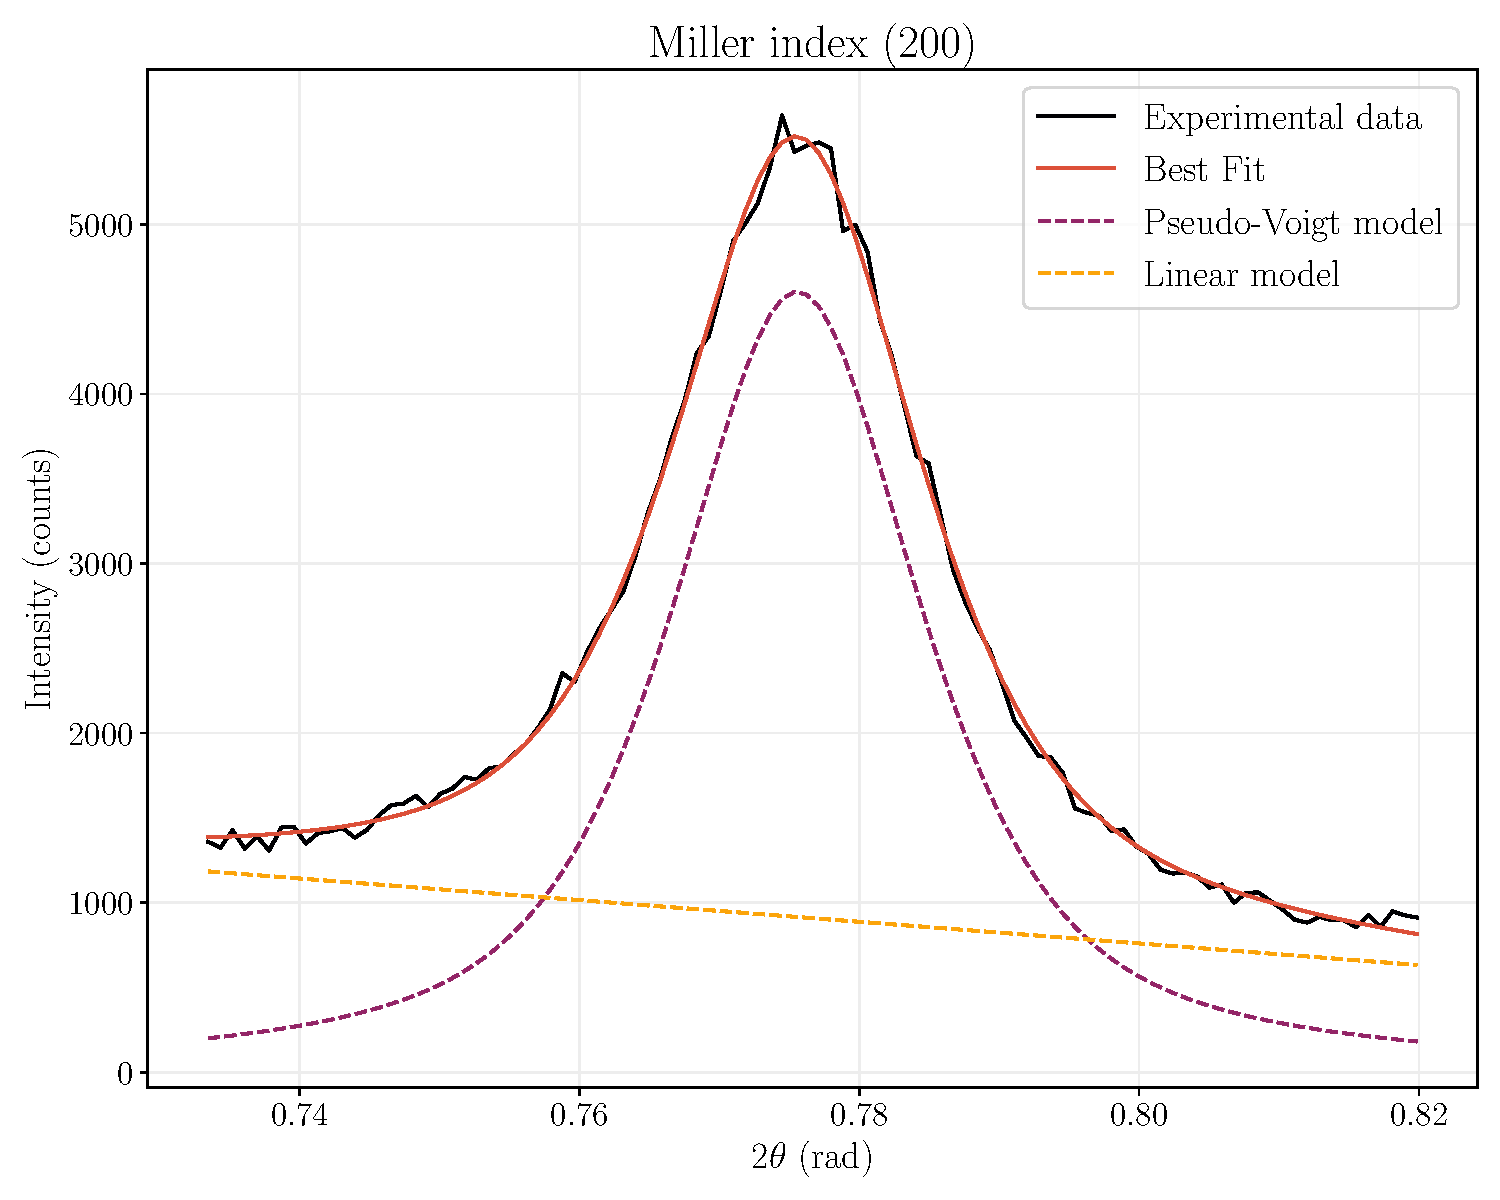
\includegraphics[width=0.3\textwidth]{images/xrd/2_peak.pdf}
    \hskip 0.01mm
   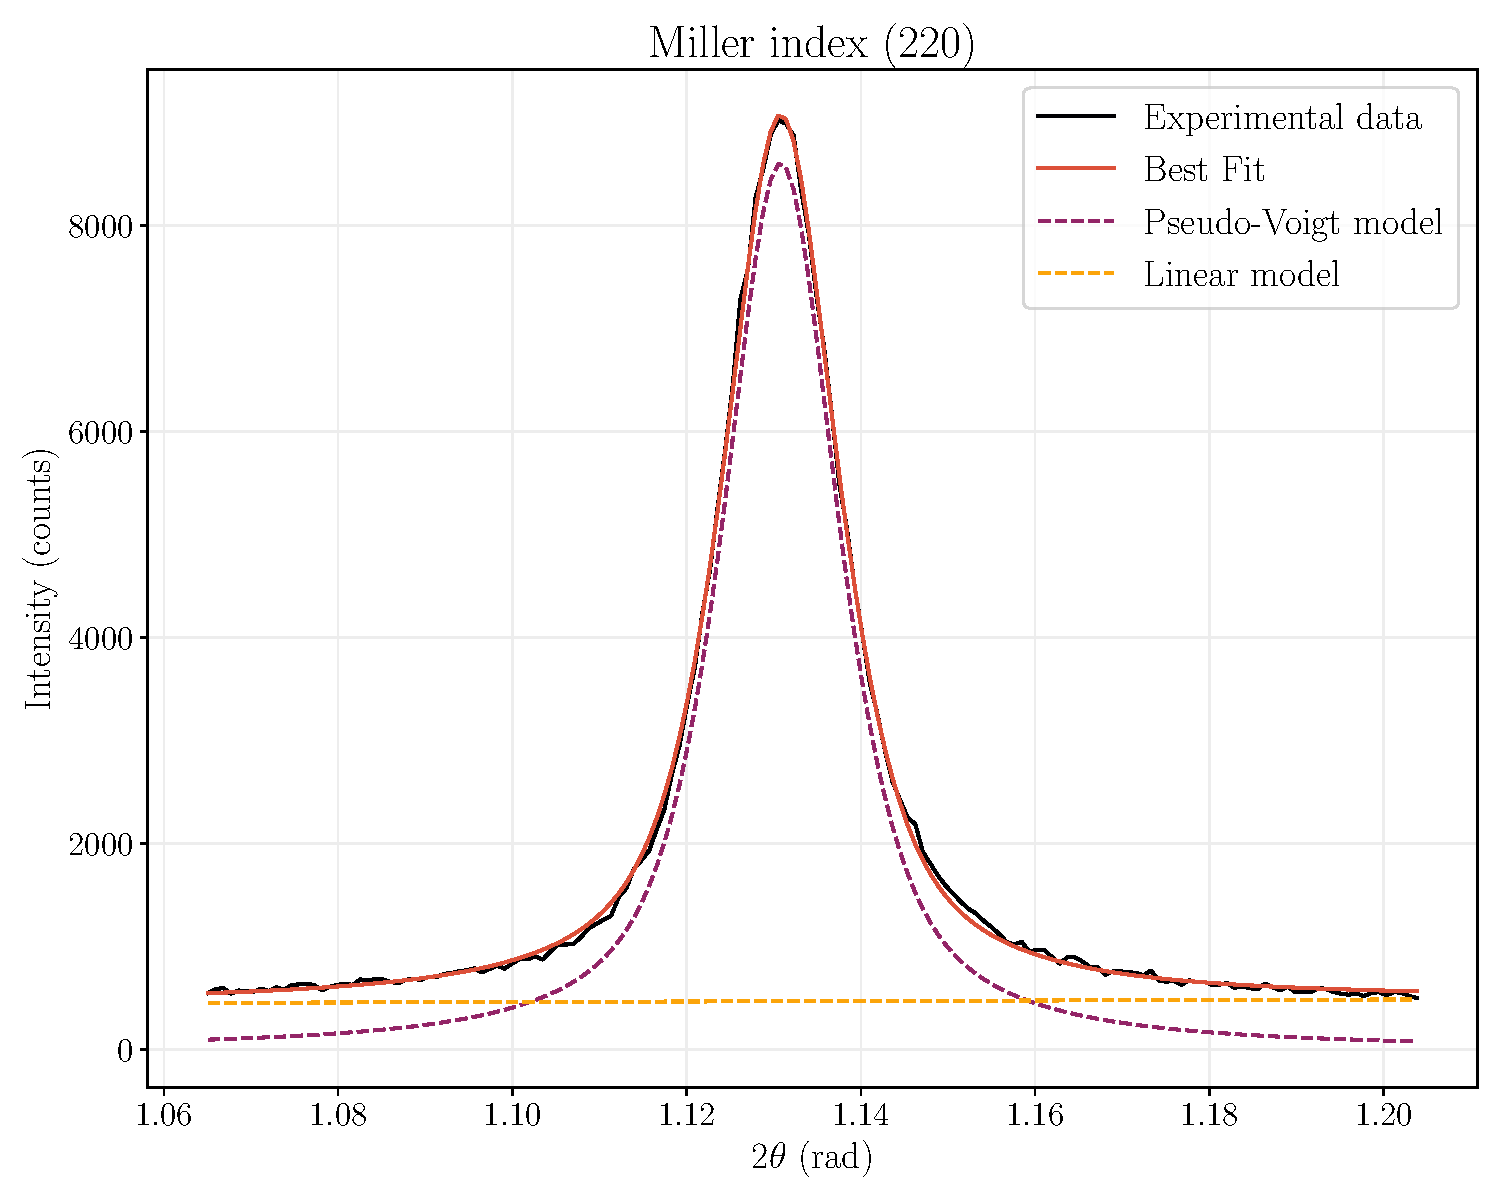
\includegraphics[width=0.3\textwidth]{images/xrd/3_peak.pdf}
   \\
   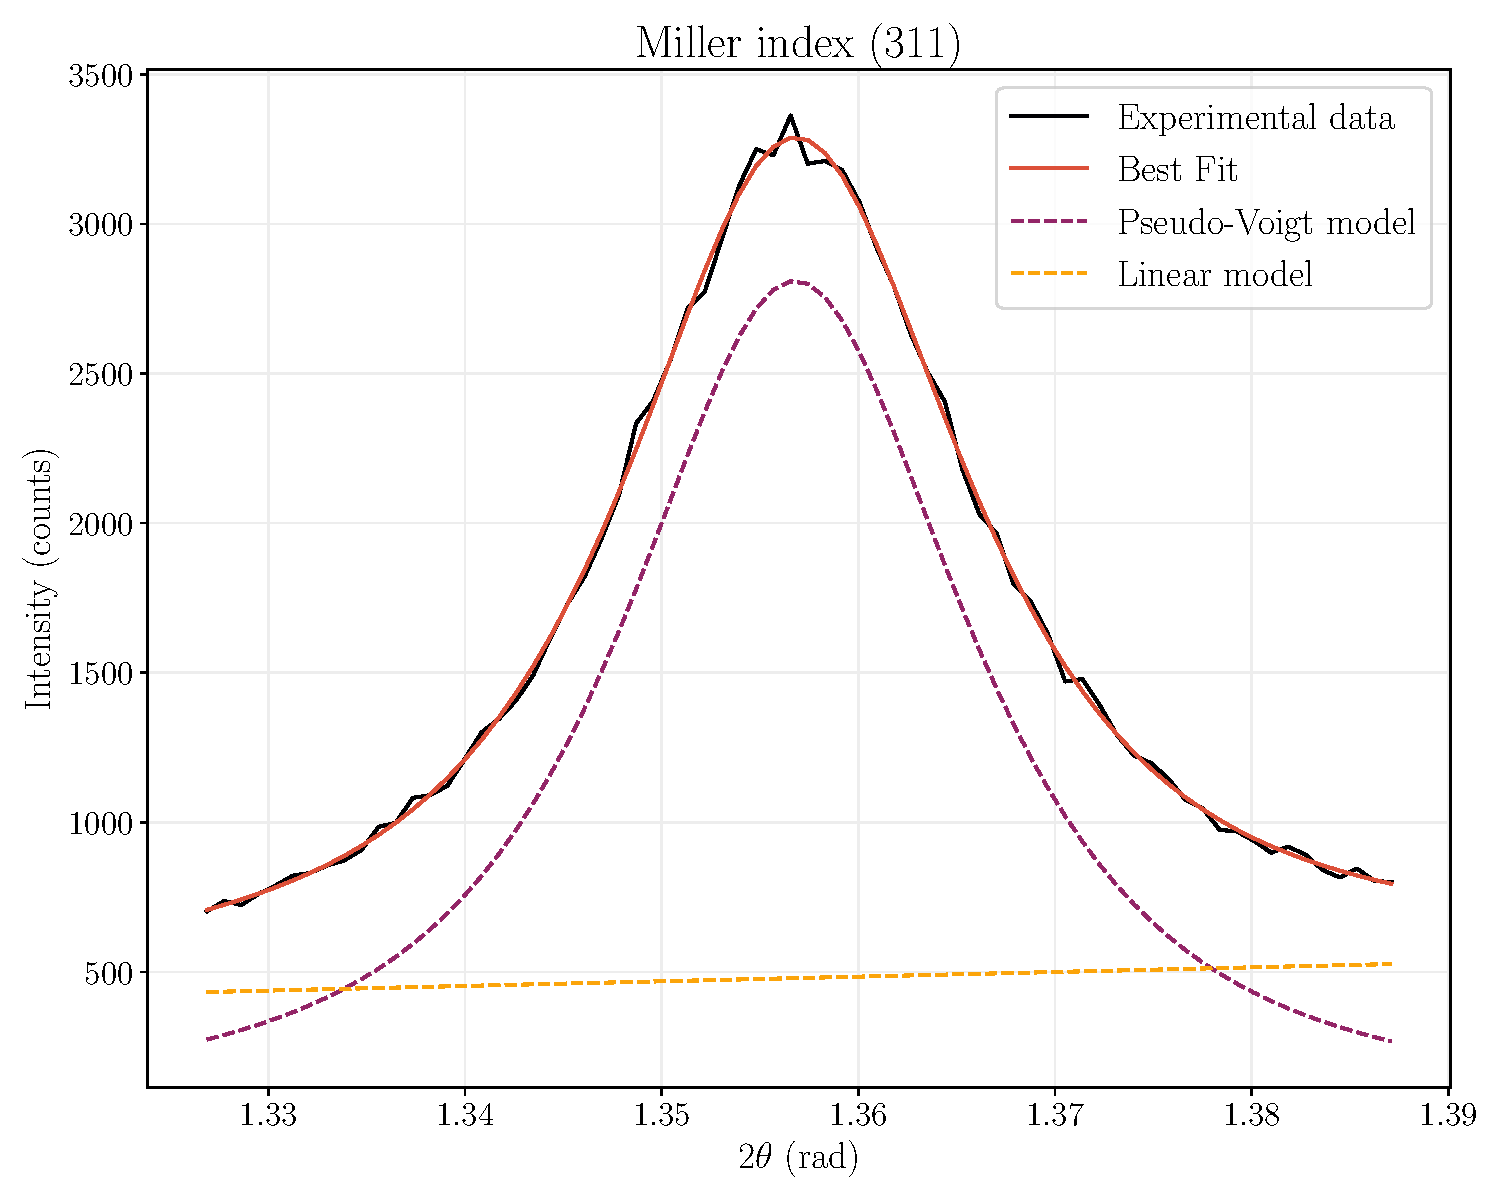
\includegraphics[width=0.3\textwidth]{images/xrd/4_peak.pdf}
   \hskip 0.01mm
   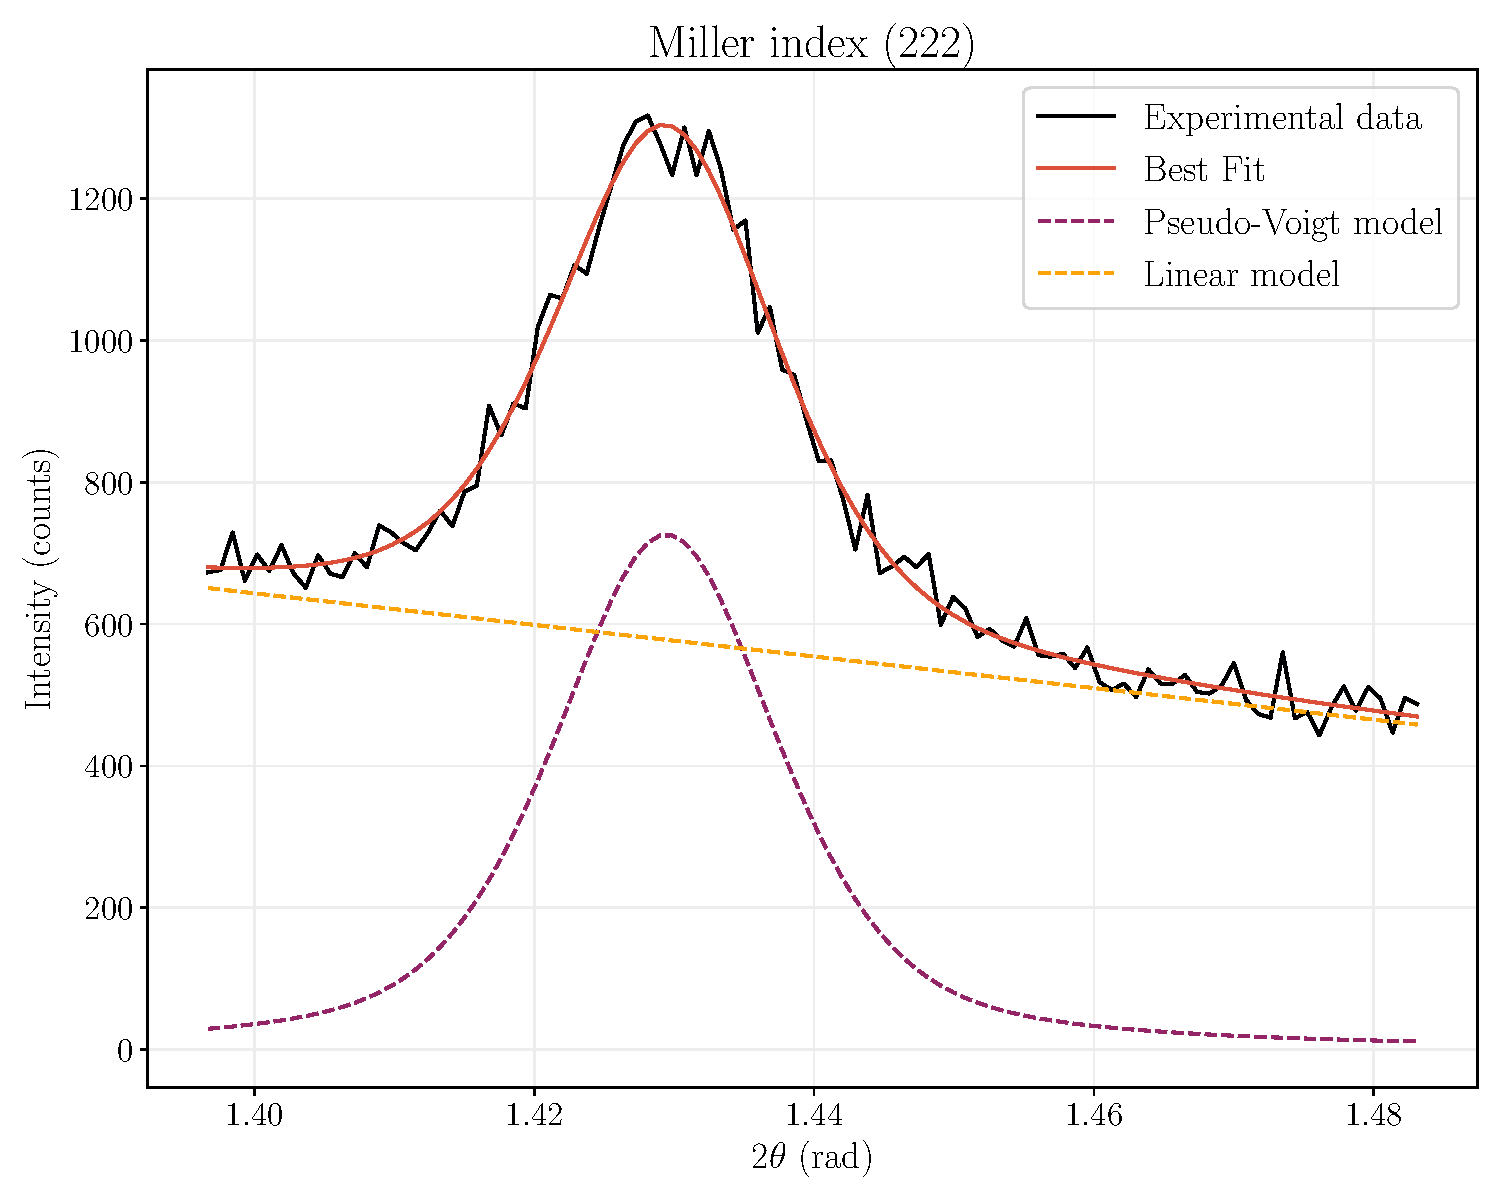
\includegraphics[width=0.3\textwidth]{images/xrd/5_peak.pdf}
   
    \caption{Fit of each of five peaks of experimental scattering intensity. The smooth lines represent the experimental data and best fit result, while the dashed lines represent the signal (Pseudo-Voigt model) and the background (linear model) separately.}
    \label{fig:peaks}
\end{figure*}

After that, we fit each experimental peak of  scattered intensity to find its center, height and Full Width Half Maximum (FHWM). 
We build a composite fit model by summing a linear model, to take into account the background noise, and a Pseudo-Voigt model to fit the effective signal. 
In particular, the Pseudo-Voigt model is defined as:
\begin{equation}
\begin{split}
f(x; A, \mu, \sigma, \alpha) 
= & \frac{(1-\alpha)A}{\sigma_g \sqrt{2 \pi}}
\exp{[ - (x-\mu)^2/ 2 \sigma_g^2 ]}  \\
&+ \frac{\alpha A}{\pi}
\qty[ \frac{\sigma}{(x-\mu)^2 + \sigma^2 } ]
\end{split}
\end{equation}
where \( \sigma_g = \sigma/ \sqrt{2 \ln 2}\). It is a weighted sum of a Gaussian and Lorentzian distribution function that share values for amplitude \(A\), center \(\mu\) and full width at half maximum.
The parameter \( \alpha \) controls the relative weight of the Gaussian and Lorentzian components.



To verify that the diffraction spectrum measured comes from gold structures, we compute the gold lattice parameter and we compare it with the bulk experimental one: \(a=0.408\,  \text{nm}\).
First of all, using the Bragg law, we compute the inter-planar spacing corresponding to each peak as:
\begin{equation}
d = \frac{\lambda}{2 \sin \theta_c}
\end{equation} 
where \(\theta_{\text{c}}\) is the position (in radians) of the peaks.
Then, we compute the lattice parameter of the phase assuming f.c.c. structure as:
\begin{equation}
a = d_{hkl} \times (h^2+k^2+l^2 )^{1/2}
\end{equation}
where \(h,k,l\) are the Miller indexes corresponding to each peak.




We can now compute the nanoparticle size from the peak broadening $\beta$ of each peak. We use the Scherrer formula, which relates the resonance peaks, occurring at angles \(2 \theta_{\text{c}} \), to the volume-weighted crystallite size \(D\):
\begin{equation}
D_V = K \frac{\lambda}{\beta \cos \theta_{\text{c}}}
\end{equation}
where \(K\) is the Scherrer constant which is shape dependent.
The most important parameter is \(\beta\) which can be defined in two different ways:
\begin{itemize}
\item as the integral breadth (\(\beta_{\text{breadth}}\)) of a reflection located at \(2\theta_c\), defined as area divided the height of the peak;
\item as the full width half maximum of the peak  (\(\beta_{\text{FWHM}}\)).
\end{itemize}
The values of the Scherrer constant, for spherical nanoparticles and according to the definitions of \(\beta\) adopted, are reported in Tab.\ref{tab:K_values}.

\begin{table}[H]
\centering
\begin{tabular*}{\columnwidth}{@{\extracolsep{\fill}}lcc}
\toprule
\textbf{Shape} & $\pmb{K}$  &  $\pmb{K}$  \\
	   & ( \(\beta\) from Integral Breadth) & (\(\beta\) from FWHM) \\
\colrule
sphere & 1.07 & 0.89 \\	   
\botrule
\end{tabular*}
\caption{Scherrer constant values.}
\label{tab:K_values}
\end{table}

\noindent In real experiments,we must take into account that the observed broadening \(\beta_{obs}\) parameter is composed by the size broadening \(\beta_{\text{size}}\) (previously defined) and the instrumental broadening \(\beta_{\text{inst}}\), as the collimation of the beam is not perfect.
We merge these two contributions in the following way: 
\begin{equation}
\beta_{\text{obs}} =\beta_{\text{inst}} + \beta_{\text{size}}
\end{equation}
The \( \beta_{\text{inst}}\)  is calibrated for our system using \(\text{LaB}_6\), supposing that only the radiation \(\text{Cu}_{ \text{k} \alpha 1 } \) with \(\lambda=0.154 \text{nm} \) is present. The value obtained is \(\beta_{\text{inst}}=0.27^\circ\).

Moreover, we take into consideration the Williamson-Hall analysis to decouple the size broadening from the strain broadening. The Williamson-Hall relationship combining size and strain broadening is:
\begin{equation}
    \qty(\beta_{\text{obs}} - \beta_{\text{inst}}) \cos \theta_c = K \frac{\lambda}{D_V} + 4 \epsilon_{\text{str}} \sin \theta_c 
\end{equation}
From a linear fit of the data it should be possible to extract the crystallite size from the intercept and the strain from the slope. 



%\begin{subequations}
%\begin{align}
%\beta_{\text{obs}} &= \beta_{\text{inst}} + \beta_{\text{size}} \\
%\beta_{\text{obs}} &= \sqrt{ \beta_{\text{inst}}^2 + \beta_{\text{size}}^2 }
%\end{align}
%\end{subequations}




\subsection{Results}

In Fig. \ref{fig:peaks} we illustrate the scattering intensity for each of the five peaks.  We notice that the fit of the first peak, the most intense one, is less affected by the noise with respect to the other four. For instance, in the fifth fit the background is quite important with respect to the signal.


In the Tab. \ref{tab:a_values} we report the results for the lattice constant $a$. The error is computed by the error propagation on $d$ as:
\begin{equation}
   \sigma_d = \frac{\lambda \cos \theta_c }{2 \sin^2 \theta_c} \sigma_{\theta_c} 
\end{equation}
where $\sigma_{\theta_c}$ is the error associated to the peak centroid by the fit. 
For all the peaks, we have a good agreement with the bulk gold constant. Thus, we have verified that the diffraction spectrum measured comes from gold f.c.c. structures.



\begin{table}[h!]
\centering
\sisetup{separate-uncertainty}
\begin{tabular*}{\columnwidth}{@{\extracolsep{\fill}}
l 
S[table-format=1.6(7)] 
S[table-format=1.5(6)] }
\toprule
\textbf{M.I.}  &  {$ \pmb{2\theta_{\text{c}} }$  (rad) } &  {$\pmb{a}$   (nm)}  \\
\colrule
111 &  0.66816 \pm 0.00003  & 0.40689 \pm 0.00001 \\
200 &  0.77556 \pm 0.00005 & 0.40742 \pm 0.00002\\
220 &  1.13081 \pm 0.00002 & 0.40667 \pm 0.00001 \\
311 &  1.3568 \pm 0.00004 & 0.40711 \pm  0.00001 \\
222 &  1.4294 \pm 0.0001 & 0.40714 \pm 0.00004  \\
\botrule
\end{tabular*}
\caption{Experimental results of Au lattice parameter for each peak.}
\label{tab:a_values}
\end{table}



In Tab. \ref{tab:xrd_result} we report the values for the size broadenings and the crystallite size for each peak. The error associated to $D_V$ is computed by the error propagation as:
\begin{equation}
    \sigma_{D_V} = K \lambda \sqrt{\qty(\frac{1}{\beta^2 \cos \theta})^2 \sigma_{\beta}^2 + \qty(\frac{\sin \theta }{\beta \cos^2 \theta})^2 \sigma_{\theta}^2 } 
\end{equation}

We observe that $D_{V_{breadth}}$ and $D_{V_{FWHM}}$ for the same peak have a nice agreement, though the values for different peaks oscillate; especially, the second peak shows a different value. We compute the weighted mean of the estimates of the five peaks. The results obtained are $D_{V_{breadth}} = (11.8 \pm 0.3) \, \text{nm}$ and $D_{V_{FWHM}}=(12.06 \pm 0.03)\, \text{nm}$, which have a good compatibility between them. 

We decide to choose as final value the one obtained from the full width half maximum, since the value of $\beta_{inst}$ we used is inherent to the $\beta_{FWHM}$.
Hence, the final radius estimate is $R = (6.03 \pm 0.02) \, \text{nm}$.


As concerns the Williamson-Hall correction, if we perform the fit in order to obtain the size broadening and the strain broadening, we see that the number of peaks is not sufficient to give a reliable fit. Hence, we decide to maintain the results from the previous analysis.


\begin{table}[H]
\sisetup{separate-uncertainty}
\begin{tabular*}{\columnwidth}{@{\extracolsep{\fill}}
l 
S[table-format=2.1(1)] 
S[table-format=2.1(2)]
S[table-format=2.1(2)]
S[table-format=2.2(3)]
}
\toprule
& { \pmb{ \( \beta_{\text{breadth}} \) } }  & { \pmb{ \( \beta_{\text{FWHM}} \) } }  & { \pmb{ \(D_{V_{\text{breadth}}} \) }} & { \pmb{ \(D_{V_{\text{FWHM}}} \) } }  \\
\textbf{M.I.} & { ($10^{-3}$rad) } & { ($10^{-3}$rad) } & { (nm) } & {(nm)} \\
\colrule
111 &  12 \pm 1  &  9.3\pm 0.1 &  14.7\pm 0.5  & 15.7\pm0.1  \\
200 & 20.8 \pm 2  & 16.5 \pm 0.2 & 8.6\pm 0.5 & 8.9\pm0.1 \\
220 &  14.5 \pm 2 & 11.3 \pm 0.1 & 13.4\pm 0.6 & 14.4\pm0.1 \\
311 &  21.2  \pm 3  &  16.4\pm 0.2 & 10.0\pm 0.7 & 10.8\pm0.2 \\
222 &  17.4  \pm 6  &  14.4 \pm 0.1  & 13 \pm 1 & 12.63\pm0.04 \\
\botrule
\end{tabular*}
\caption{Experimental results of Au lattice parameter and crystallite size for each peak.}
\label{tab:xrd_result}
\end{table}












\section{Scanning Electron Microscopy Analysis}

\subsection{Method}

At last, we perform an analysis of our sample using a Scanning Electron Microscope, in order to obtain a digital image and measure the nanoparticles size in a more direct way.

A scanning electron microscope (SEM) is an electro-optical instrument, with a typical resolution of 1 nm. It scans a focused electron beam over a surface to create an image. The electrons are produced by a source, they are accelerated through a column and focused by electromagnetic lenses; the beam hits the sample chamber and signals are collected by detectors. The column and the chamber work at a vacuum level of about $10^{-3}$ Pa.
The beam interacts with the sample and transfers its energy through phonons and plasmon production, atomic ionization and inelastic interaction with nuclei. The signals collected are secondary electrons, back-scattered electrons and the X-rays spectrum.

In Fig.\ref{fig:sem_image} the four SEM images are illustrated. 
In particular, each image has its own resolution, that can be deduced by the information on the pixel size, reported on the image itself.

We analyze them through the software “ImageJ”, which is able to recognize the single particles. First of all, for each image, we make sure to manually exclude the particles at the boundary, which are not fully represented in the picture and would spoil the results, and we also exclude the aggregated nanoparticles. 




\begin{figure*}[htp]
    \centering 
    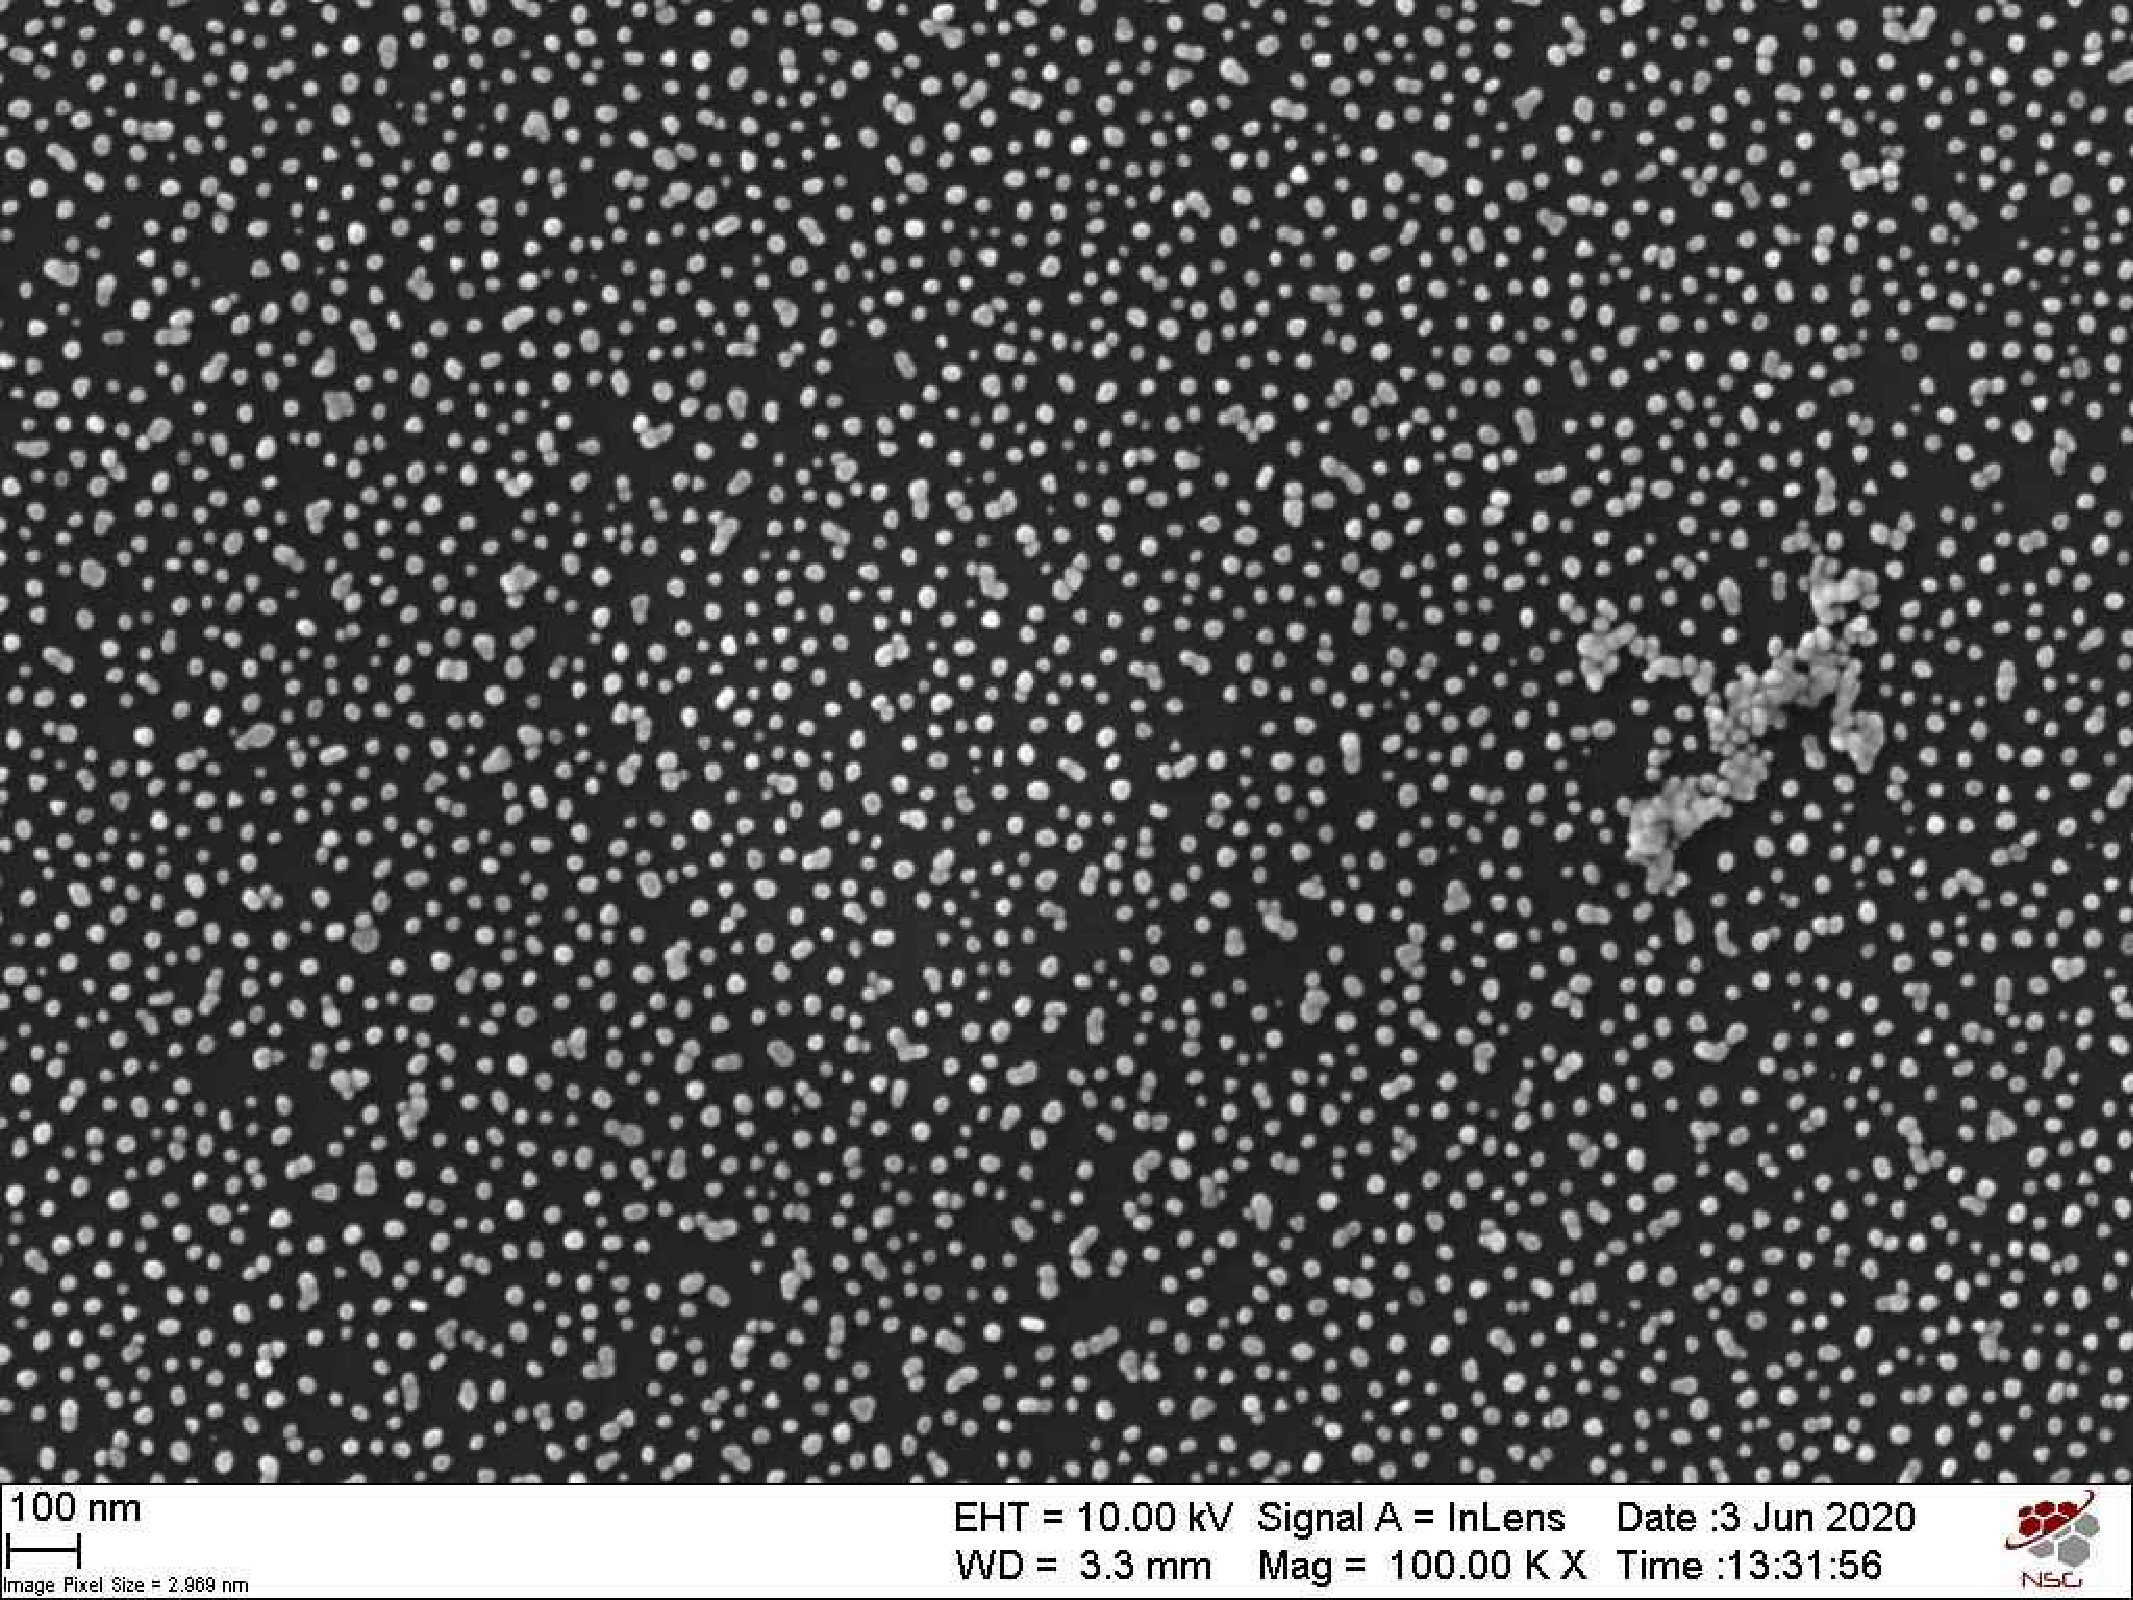
\includegraphics[width=0.47\textwidth]{images/sem/AuNP_05.pdf}
    \hskip 0.01mm
    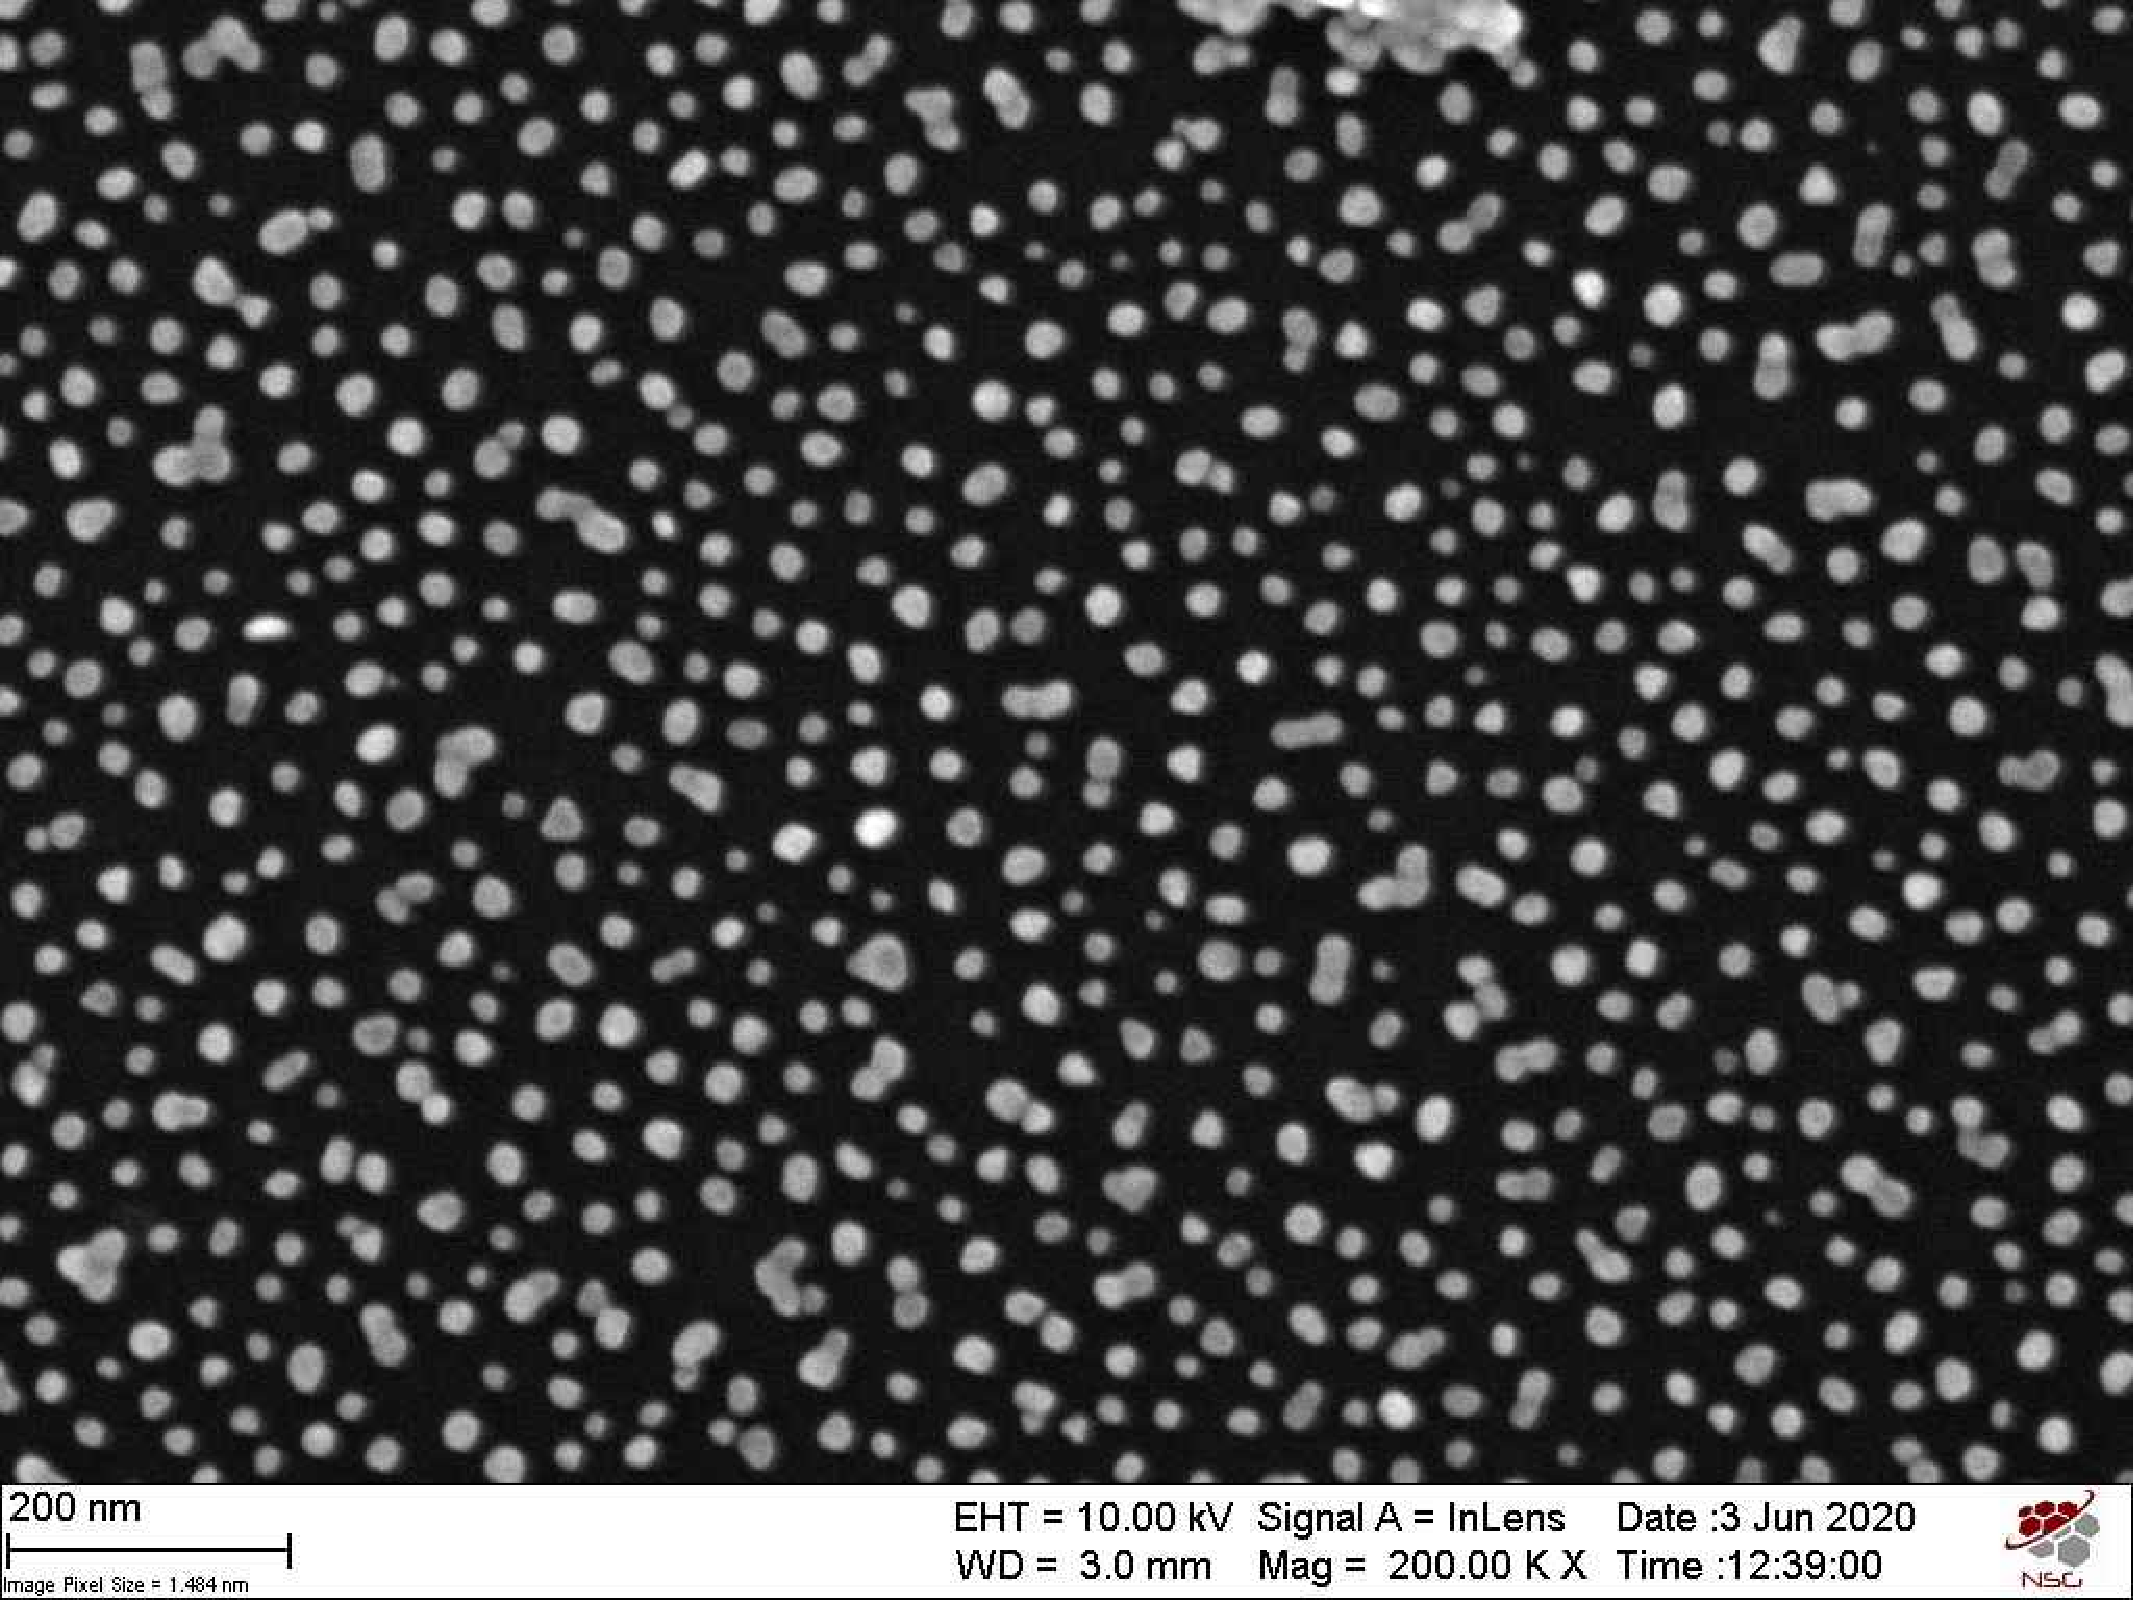
\includegraphics[width=0.47\textwidth]{images/sem/AuNP_01.pdf}
    \hskip 0.01mm \\
    \vskip 0.3 mm
    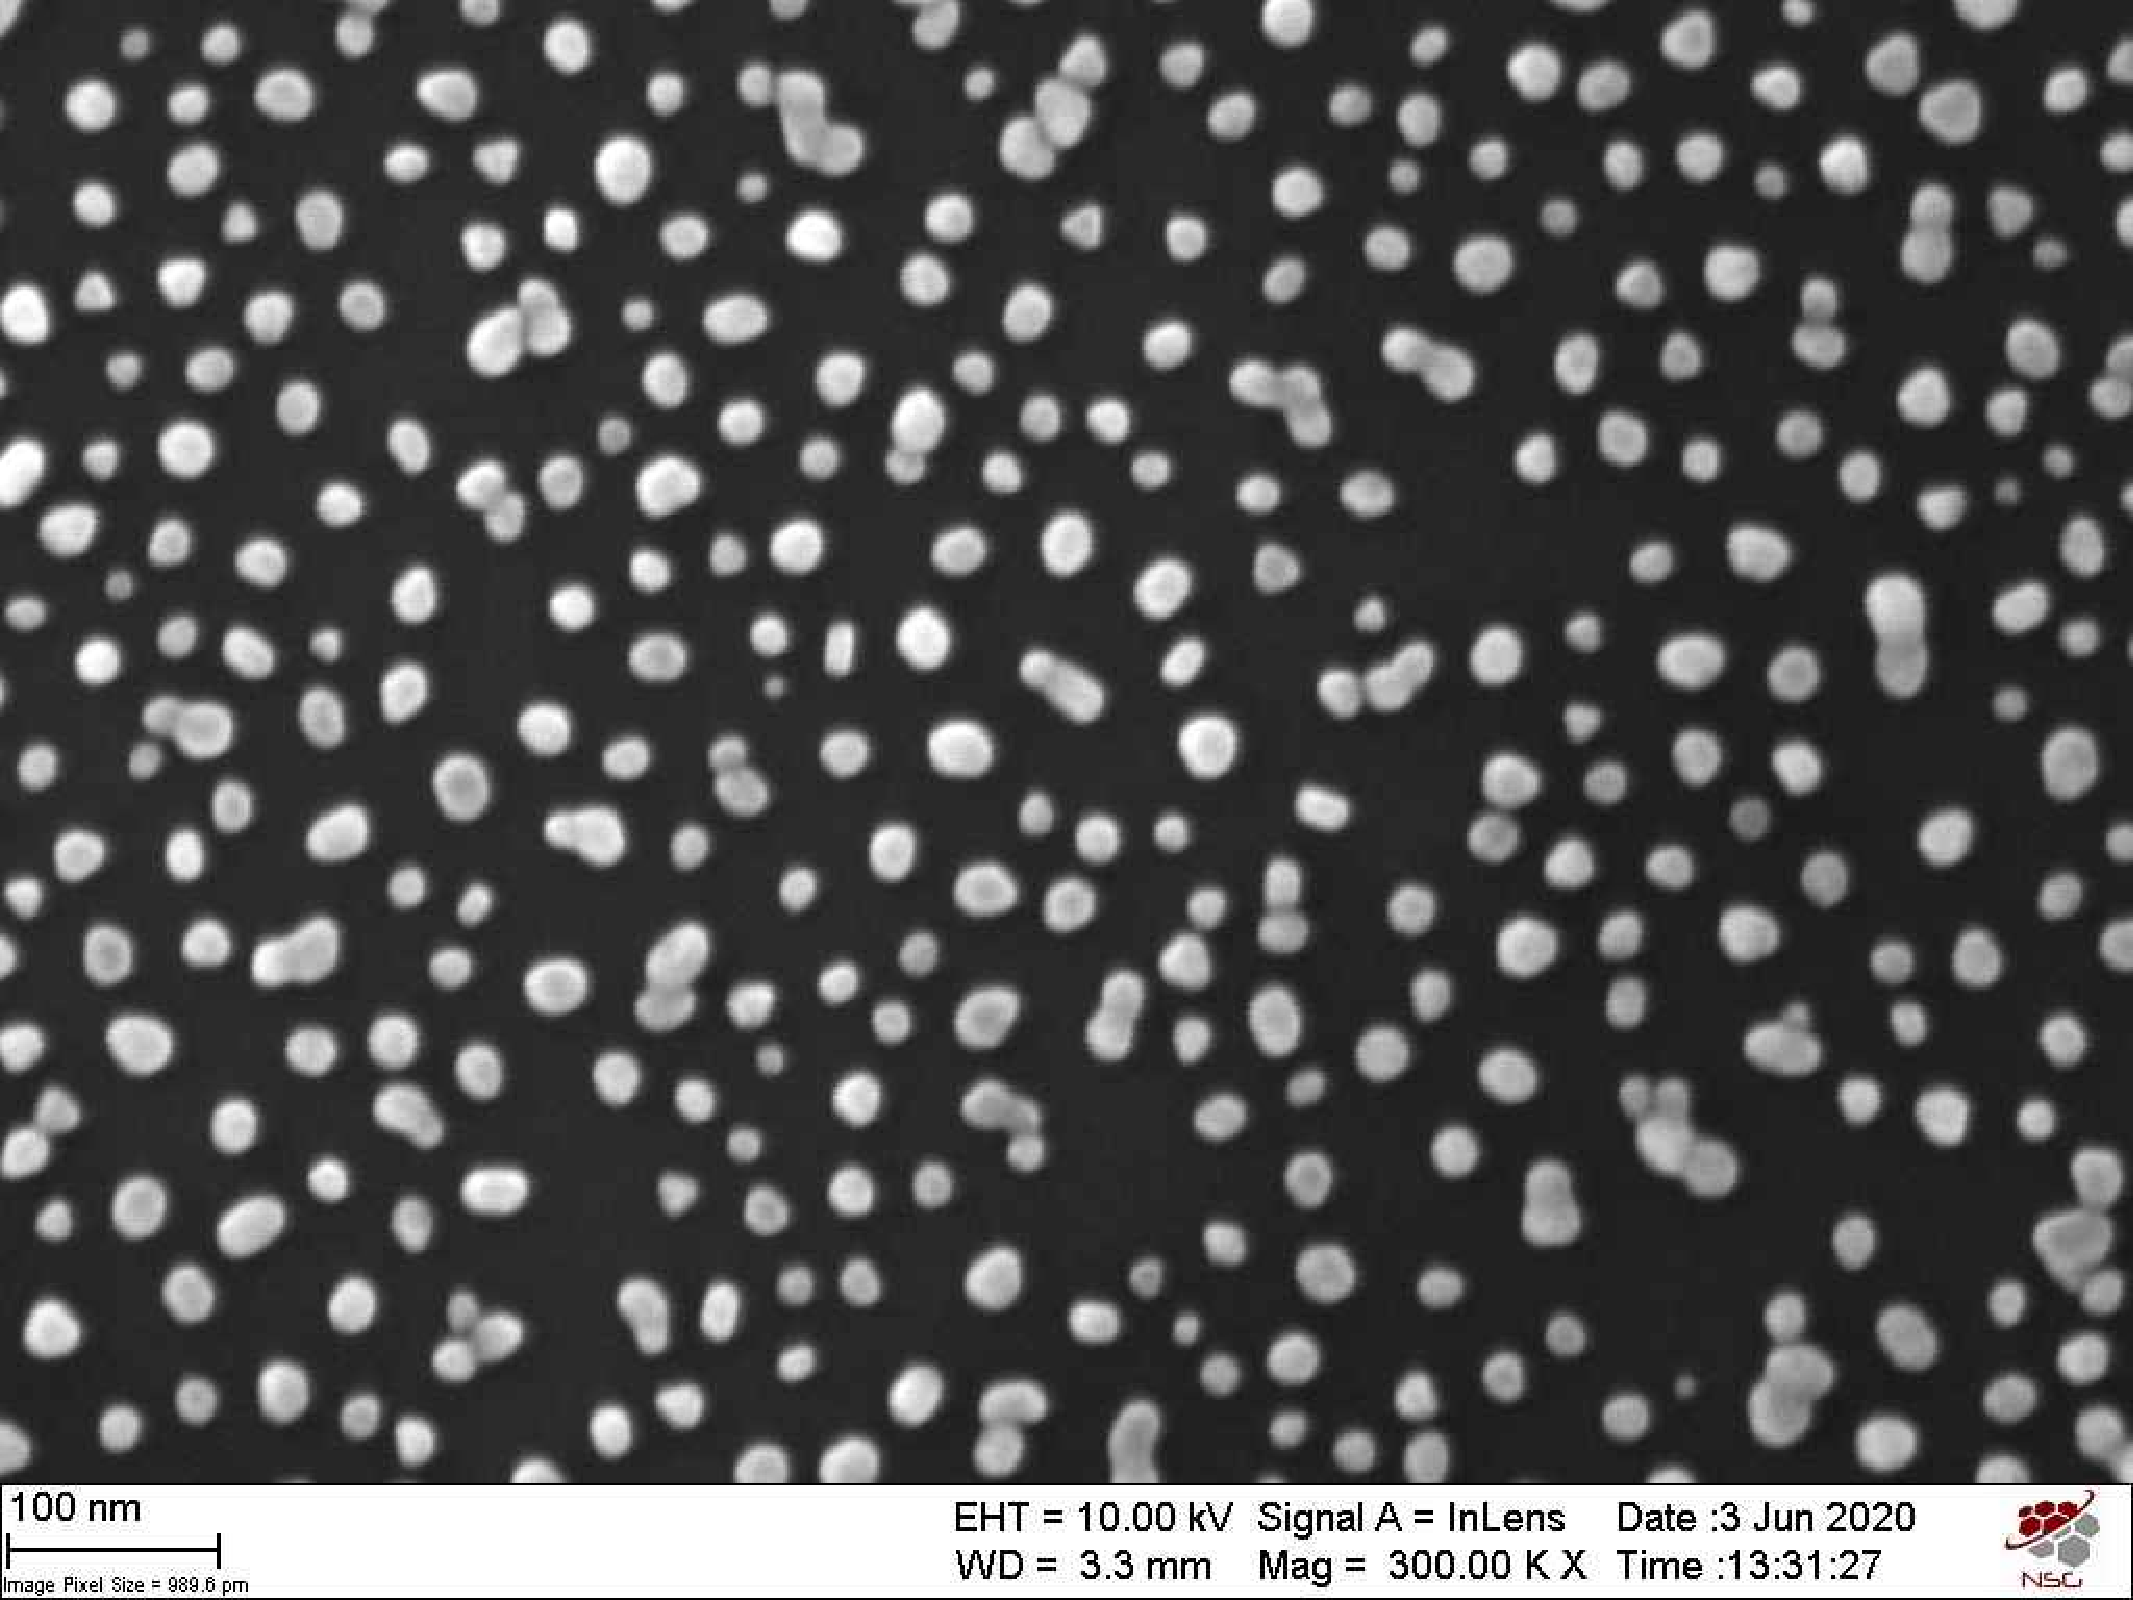
\includegraphics[width=0.47\textwidth]{images/sem/AuNP_04.pdf}
    \hskip 0.01mm
    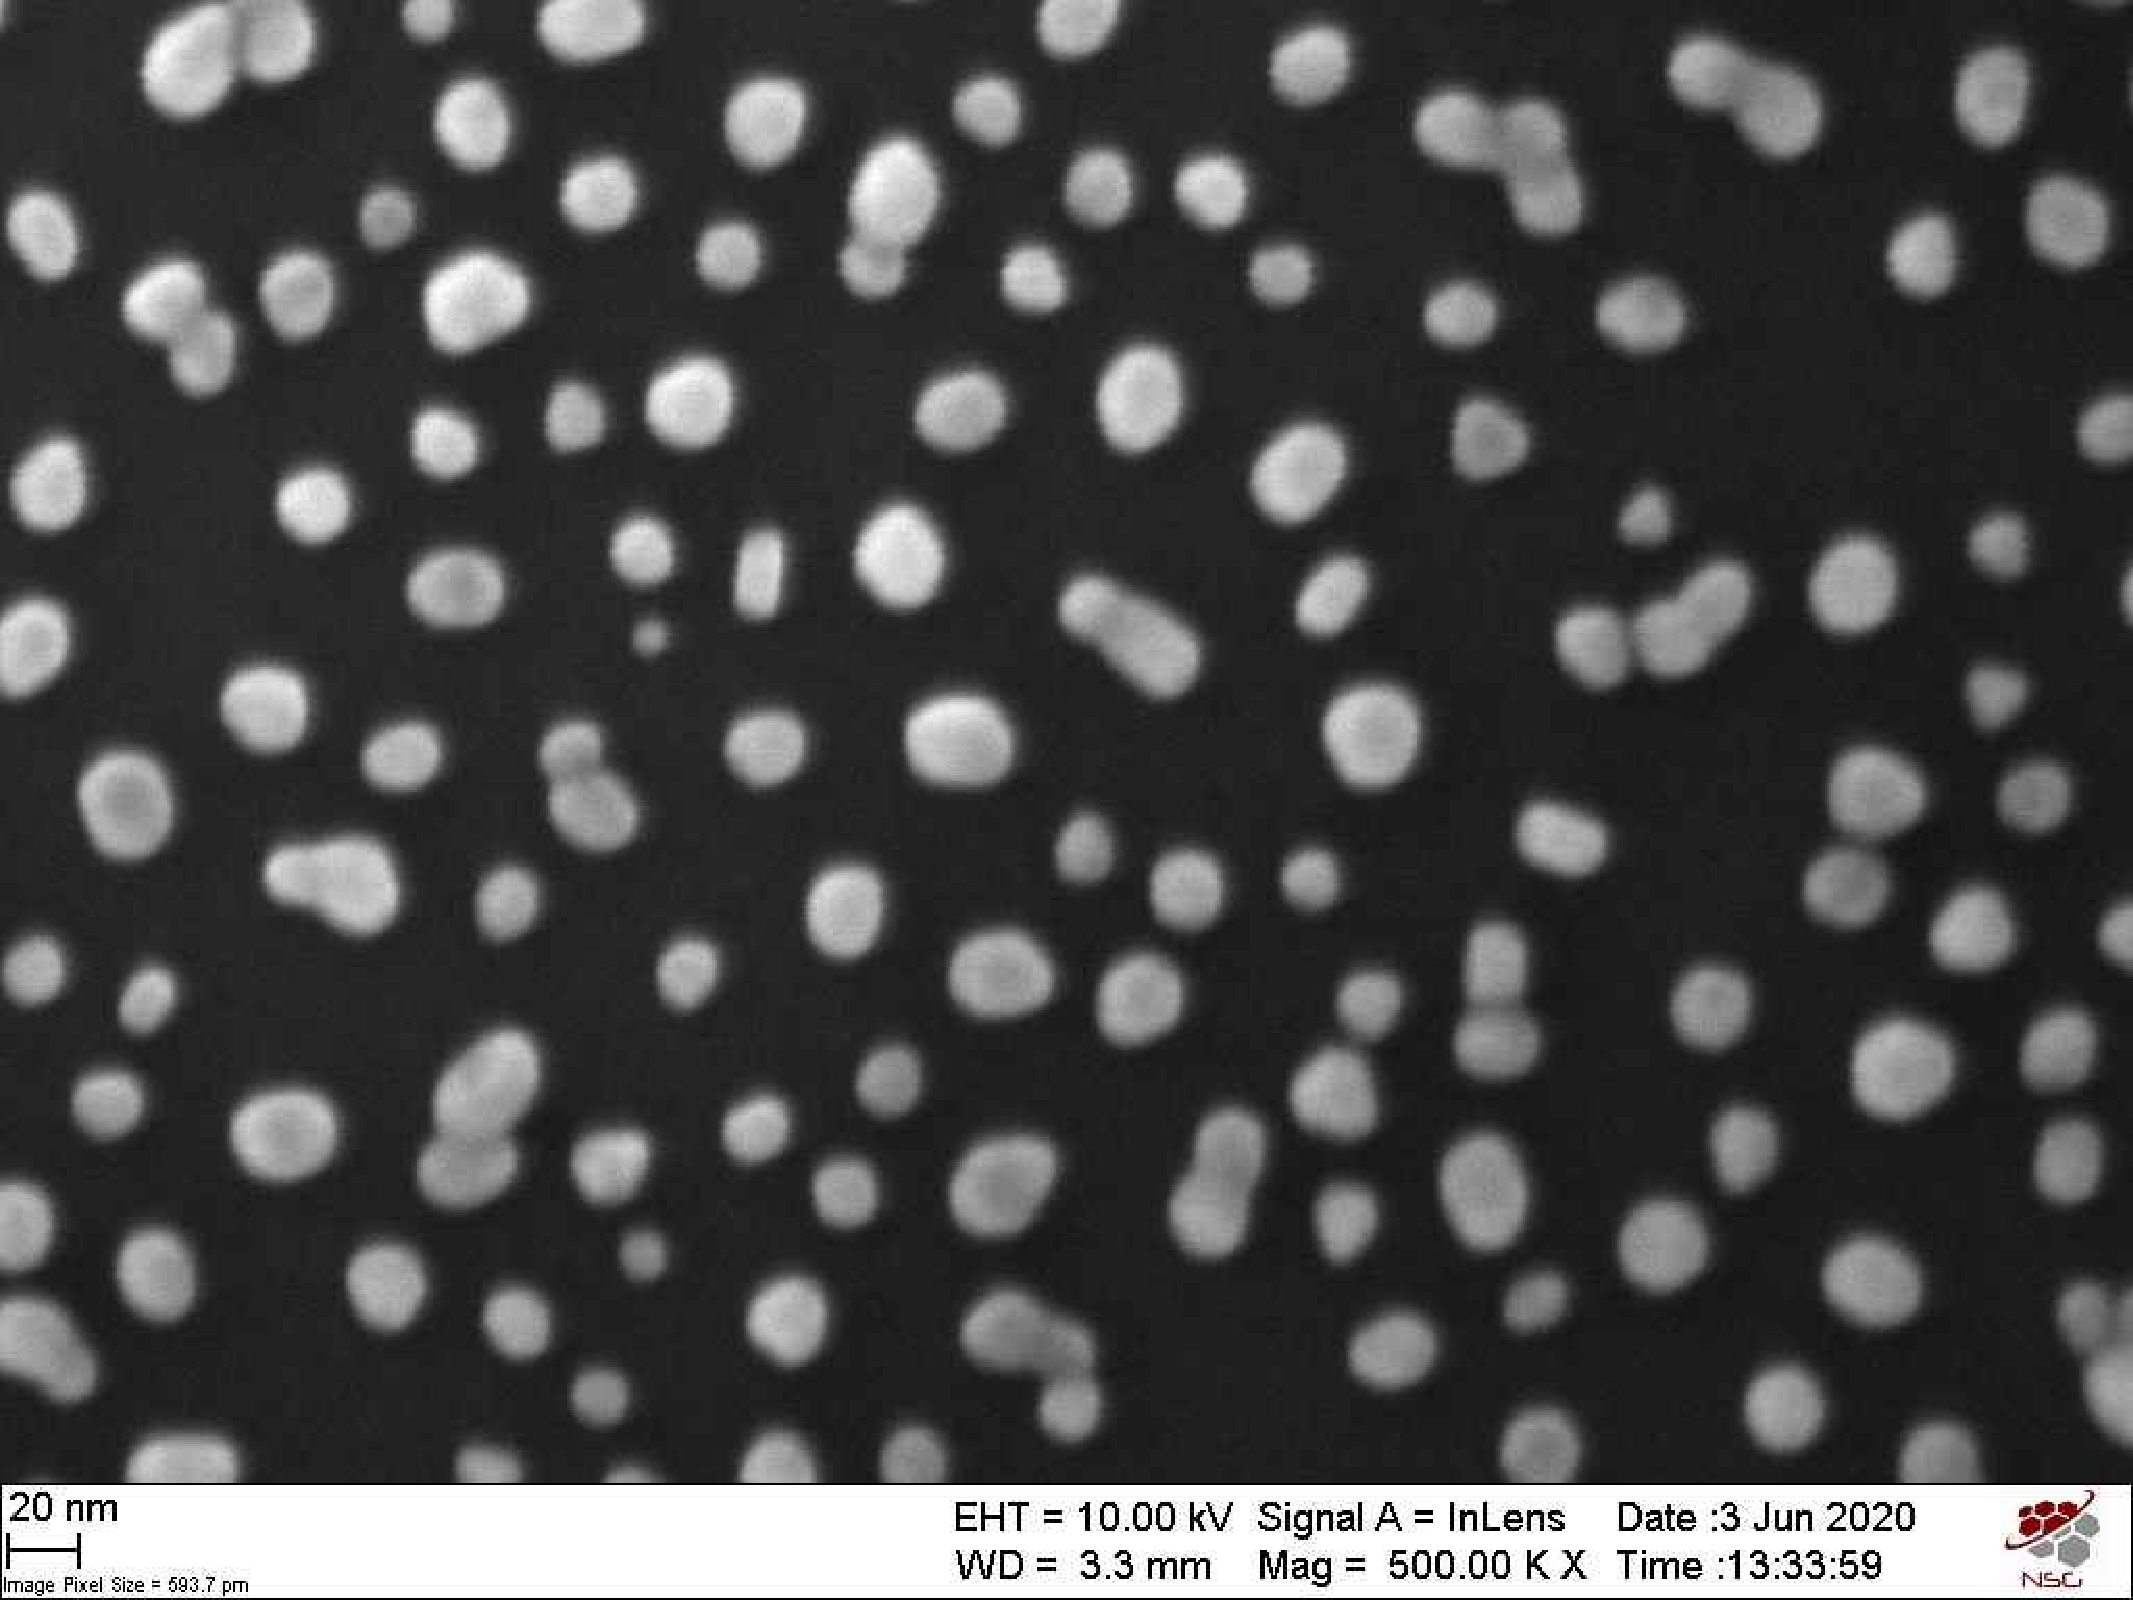
\includegraphics[width=0.47\textwidth]{images/sem/AuNP_07.pdf}
    \caption{Images acquired by Scanning Electron Microscope. The four images have a different scale and a different resolution. }
    \label{fig:sem_image}
\end{figure*}

Then, for each image, we collect the measure of the surface area $A$, major and minor axis ($a_1$ and $a_2$) of each particle.

We estimate the effective radius as $R_{eff} = \sqrt{A/\pi}$ and the aspect ratio of the ellipsoidal nanoparticles, $a_r = a_1/a_2$. Then, we make a histogram of the aspect ratio values in order to verify if it contains extreme values. Moreover, we make a histogram of the effective radius  $R_{eff}$ and we fit it with a lognormal probability density function, previously defined in Eq.\ref{eqn:log_normal}. 

We compute the mean of the distribution as $\expval{R_{eff}} = \exp(\mu+\sigma^2/2)$ and its associated error by propagation of uncertainty. 

Furthermore, since from the previous experiments we obtain information coming from the nanoparticle volume, the size we obtain is $\sqrt[3]{\expval{r^3}}$. In order to compare the SEM estimates with the previous ones, we must compute the cubic root of the third moment of the distribution. Hence, we compute the third moment analytically as: 
\begin{equation}
    \expval{R_{eff}^3} = e^{3 \mu+  \frac{9 \sigma^2}{2}}
\end{equation}
and then we take {\scriptsize{$\sqrt{\expval{R_{eff}^3}}$}}.
Also in this case the error is computed by propagation of uncertainty.



\subsection{Results}

In Tab.\ref{tab:sem_experimental_data} we report the average measurements referred to each dataset coming from a single SEM image.

\begin{table}[h!]
\sisetup{separate-uncertainty}
\begin{tabular*}{\columnwidth}{@{\extracolsep{\fill}}
S[table-format=1.4(0)] 
S[table-format=3.2(2)] 
S[table-format=2.2(2)]
S[table-format=2.2(2)] }
\toprule
\textbf{Pixel Size}& { \textbf{Area} }  & { \pmb{$a_1$}}  & { \pmb{$a_2$}} \\
 { (nm) } & { ($\text{nm}^2$) } & { (nm) } & {(nm)} \\
\colrule
2.969 &  392.30 \pm 0.02  &  24.12 \pm 0.02 &  19.99 \pm 0.02  \\
1.484 & 395.52 \pm 0.02  & 23.98 \pm 0.02 & 20.29 \pm  0.02  \\
0.9896 &  384.08 \pm 0.02 & 23.51 \pm 0.02 & 20.03 \pm  0.02 \\
0.5937 &  400.11  \pm 0.03 &  24.22 \pm 0.02  & 20.15 \pm 0.02 \\
\botrule
\end{tabular*}
\caption{Average of experimental results for each SEM dataset which is denoted by the pixel size.}
\label{tab:sem_experimental_data}
\end{table}

At first, we analyze each dataset coming from one image individually and we obtain the average effective radius and aspect ratio with the associated weighted mean error. The results are reported in Tab.\ref{tab:sem_results}. 
From the aspect ratio estimates, we observe that in average the particles shape slightly deviates from the spherical one in all the four datasets. 
We join all the aspect ratio measurements in the histogram in Fig.\ref{fig:histogram_ar}. We notice that this histogram has a tail for events with high $a_r$: this may indicate that we included by mistake in the analysis some aggregated particle which apparently form an elongated ellipse. However, they are a few and they should not affect the statistics.

\begin{table}[h!]
\sisetup{separate-uncertainty}
\begin{tabular*}{\columnwidth}{@{\extracolsep{\fill}}
S[table-format=1.4(0)] 
S[table-format=2.5(6)] 
S[table-format=2.2(2)]}
\toprule
\textbf{Pixel Size}& {\pmb{$R_{eff}$} }  & { \pmb{$a_r$}} \\
 { (nm) } & { (nm) } &  \\
\colrule
2.969 & 11.7639 \pm 0.0004 & 1.21 \pm 0.02 \\
1.484 & 11.8032 \pm 0.0002 & 1.18 \pm 0.04 \\
0.9896 &  11.6504 \pm 0.0001 &  1.17 \pm 0.06 \\
0.5937  &  11.91073 \pm 0.00009 & 1.2 \pm 0.1 \\
\botrule
\end{tabular*}
\caption{Average of effective radius $R_{eff}$ and aspect ratio $a_r$ for each SEM dataset, which is denoted by the pixel size. The associated errors are computed as weighted mean errors.}
\label{tab:sem_results}
\end{table}




In order to perform the distribution fit, we decide to join all the datasets, in order to derive it with all the information we got from the measurements. 
The different datasets have a different resolution and hence a different error on the measurements. This means that the heights of the columns of the histogram are affected by an error, that can be estimated as the square root of the sum of the squared errors.


\begin{figure}[t!]
    \begin{minipage}[l]{1.0\columnwidth}
    \centering
    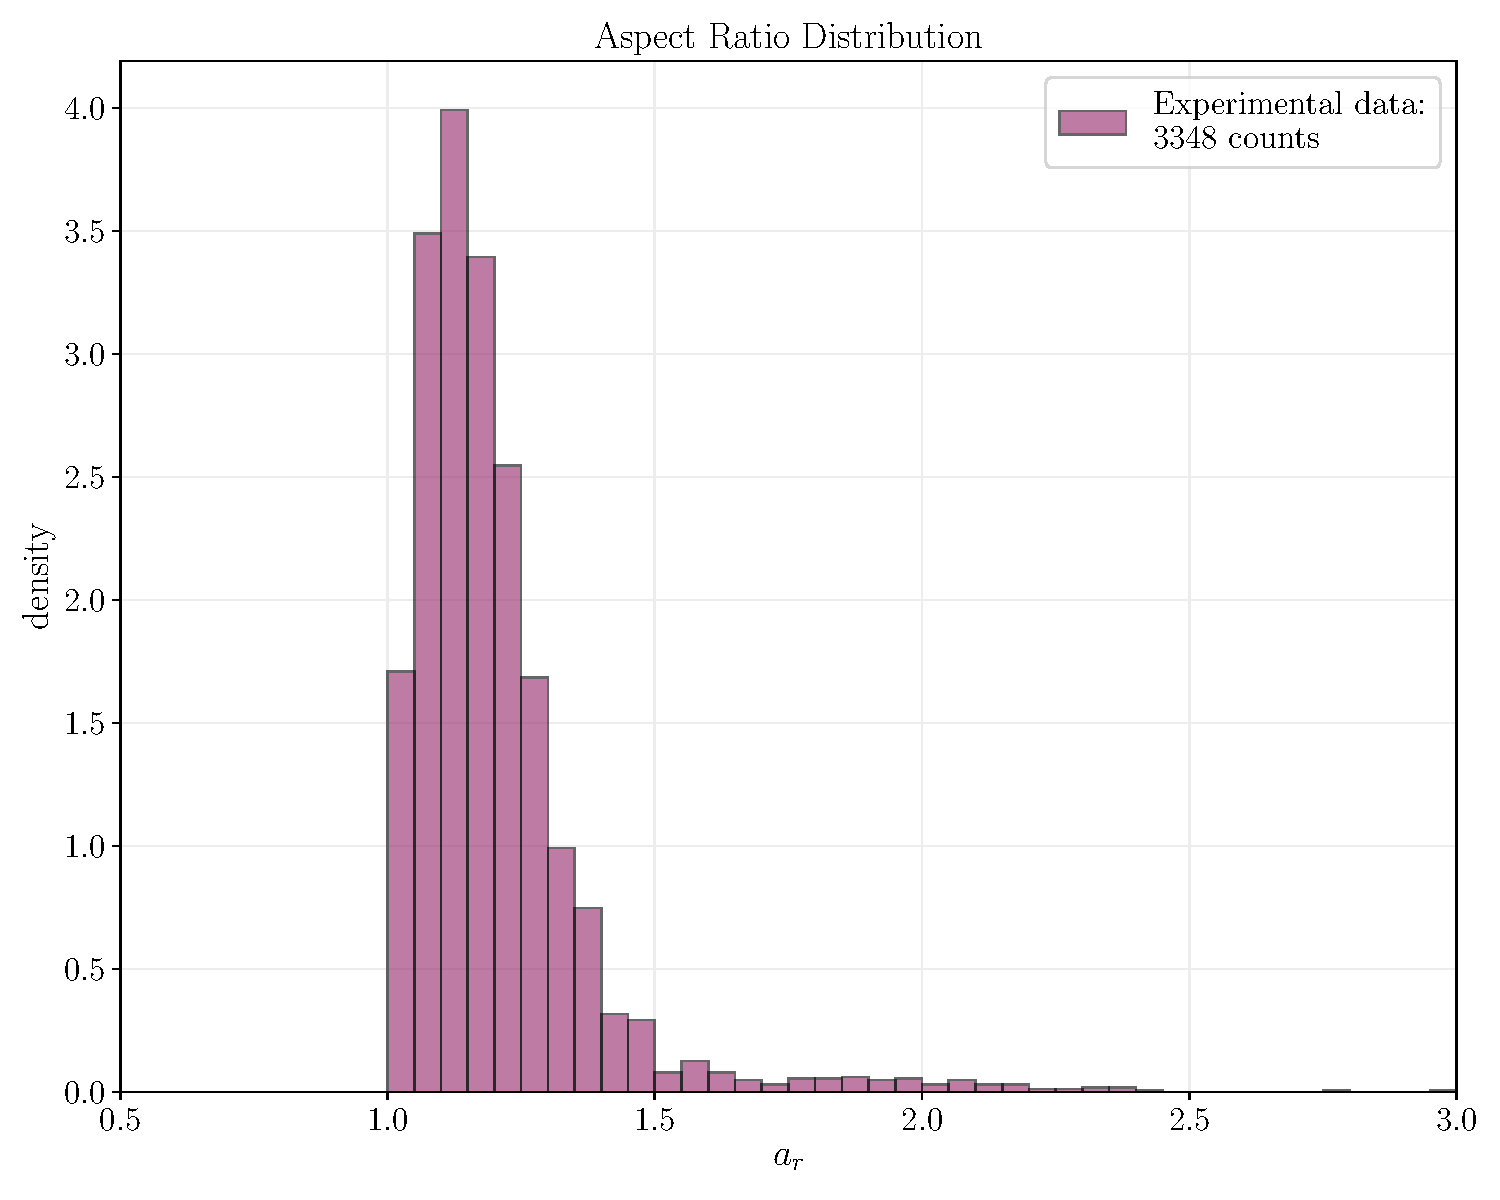
\includegraphics[width=0.9\textwidth]{images/sem/histogram_ar.pdf}
    \caption{Histogram of aspect ratio $a_{r}$. In the legend, the number of entries in the histogram is reported.}
    \label{fig:histogram_ar}
    \end{minipage}
\end{figure}

The histogram with its associated fit is illustrated in Fig.\ref{fig:histogram_fit}. In particular, the fit parameters are:
\begin{equation*}
    \mu=(2.425 \pm 0.008)\, \text{nm},  \,\, \sigma=(0.202\pm0.009) \, \text{nm}
\end{equation*}
Then, we compute the mean of the distribution and also the cubic root of its third moment, with their associated errors. The results are:
\begin{equation*}
   \expval{R_{eff}} = (11.5 \pm 0.1) \, \text{nm}, \quad {\scriptstyle \sqrt{\expval{R_{eff}^3}} }=(12.0\pm0.1) \, \text{nm}
\end{equation*}




\begin{figure}[htp]
    \begin{minipage}[l]{1.0\columnwidth}
    \centering
    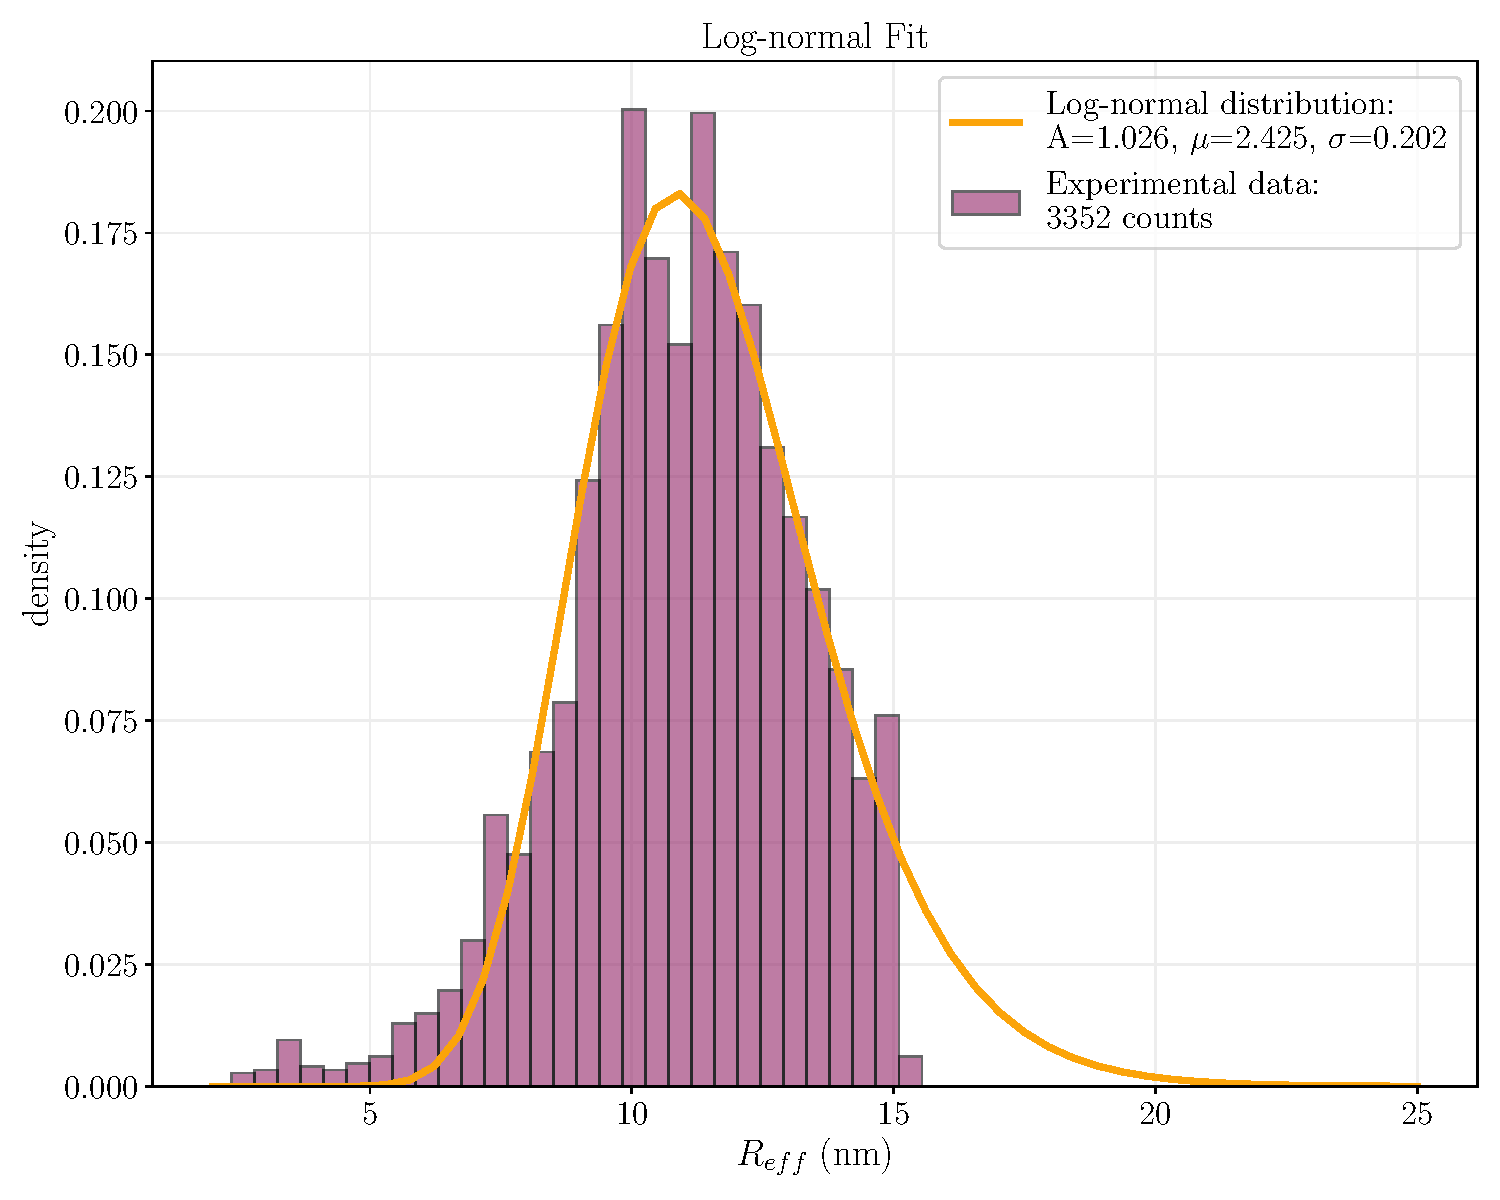
\includegraphics[width=0.9\textwidth]{images/sem/histogram_fit.pdf}
    \caption{Histogram of effective radius $R_{eff}$ with associated log-normal distribution which parameters are obtained by a fit of the histogram. In the legend, the distribution parameters and the number of entries in the histogram are reported.}
    \label{fig:histogram_fit}
    \end{minipage}
\end{figure}








%%%%%%%%%%%%%%%%%%%%%%%%%%%%%%%%%%%%%%
\section{Discussion}


We have obtained three estimates for the particle radius, or better for the cubic root of the mean value of the cube of the radius, which are reported in Table \ref{tab:R_comparison}. 



\begin{table}[H]
\sisetup{separate-uncertainty}
\begin{tabular*}{\columnwidth}{@{\extracolsep{\fill}}
c
S[table-format=2.2(3)] 
l %S[table-format=1.1(2)] 
}
\toprule
 {\pmb{Method}} & { \pmb{$\expval{R^3}^{1/3}$} (nm)} \\
 \colrule
{Optical} & 5 \pm 1    \\
{X-ray} & 6.03 \pm 0.02     \\
{SEM} &  12.0 \pm 0.1  \\
\botrule
\end{tabular*}
\caption{Nanoparticles radius estimates with the three methods.}
\label{tab:R_comparison}
\end{table}



We can clearly see that the ones from optical absorbtion and X-rays diffraction are compatible, while the SEM result is not. For sure the third value is the most reliable, since we directly “see” the particles. As concerns the X-rays method: if we rely mostly on the estimate obtained by the peak $(1 1 1)$ of the spectrum, which is the less affected by statistical error, we get a value of the radius of $7.9 \pm 0.1$ nm, which is closer to the SEM estimate. 
As regards the first method, we obtained a radius value with quite high uncertainty, since the fit quality is not so sensitive with respect to the change of parameters, or with respect to the introduction of a size-dispersed system. Moreover, the value obtained for $\epsilon_m = 2.1 \pm 0.1$ means that the value for the refractive index of the medium is $n_m = 1.45$, whereas we expect a value similiar to $n_{\text{water}} = 1.33$. This suggests some problems in this method.

\begin{figure*}[t!]
    \centering 
    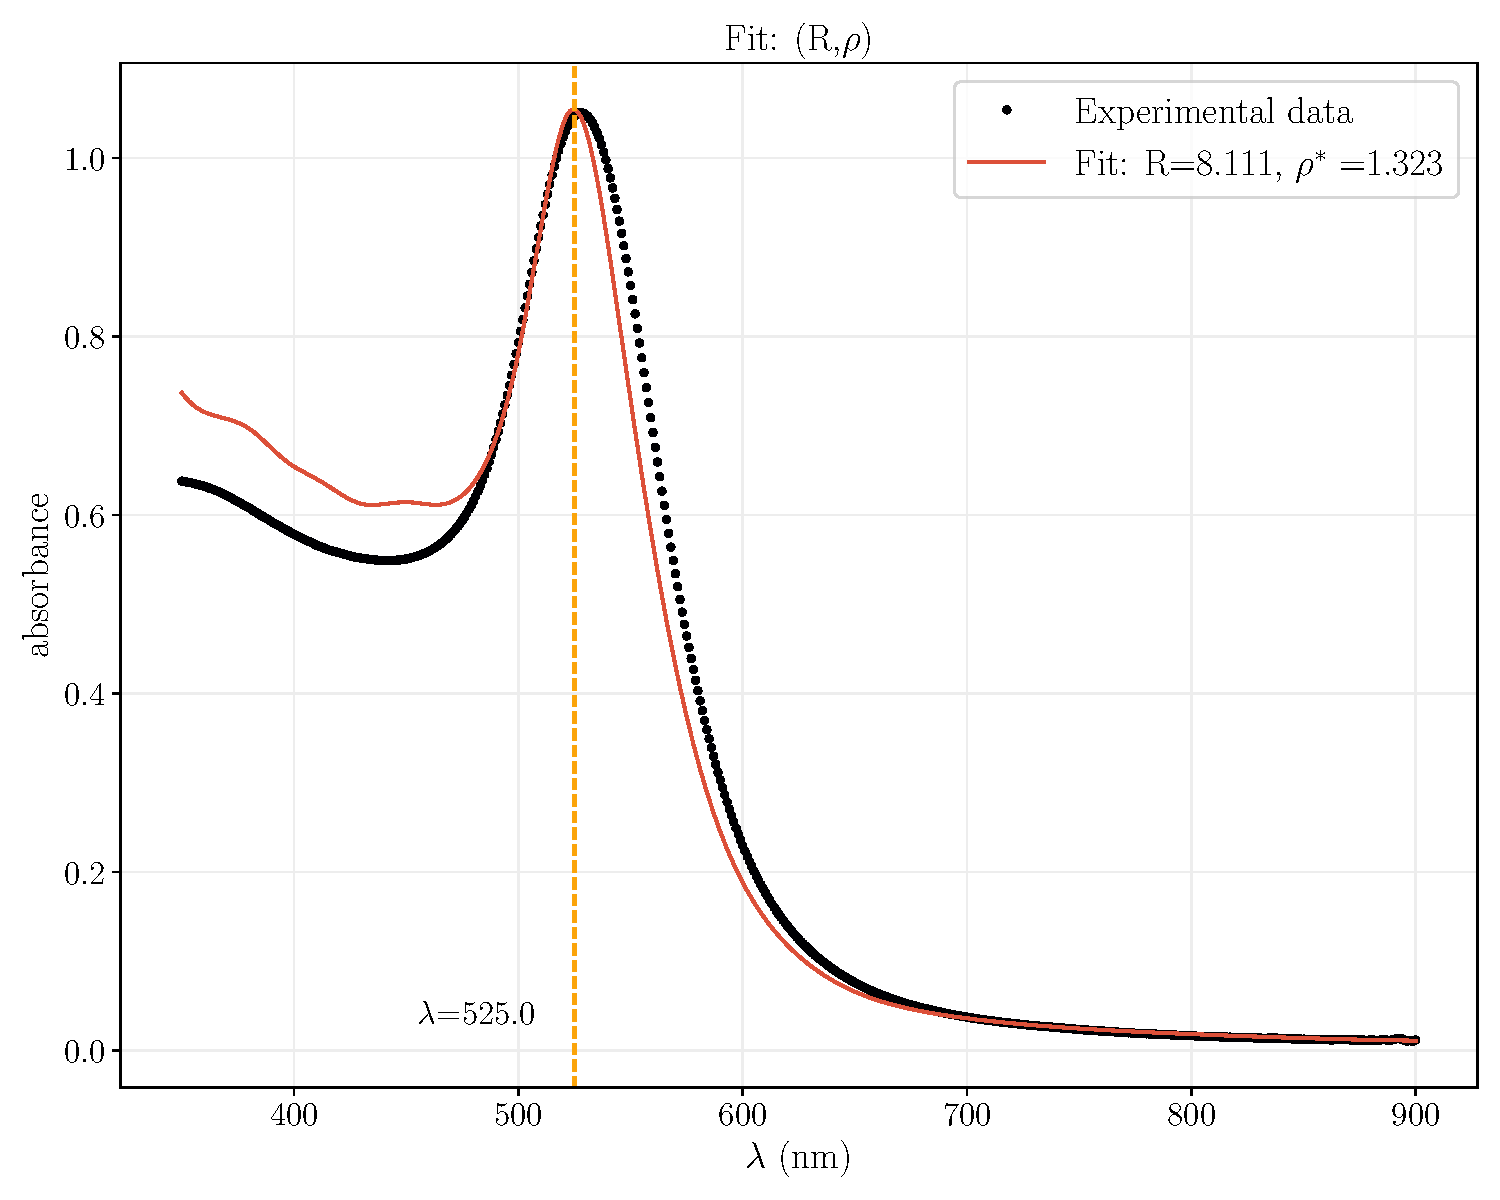
\includegraphics[width=0.49\textwidth]{images/os/1_fit_GANS.pdf}
    \hskip 1mm
   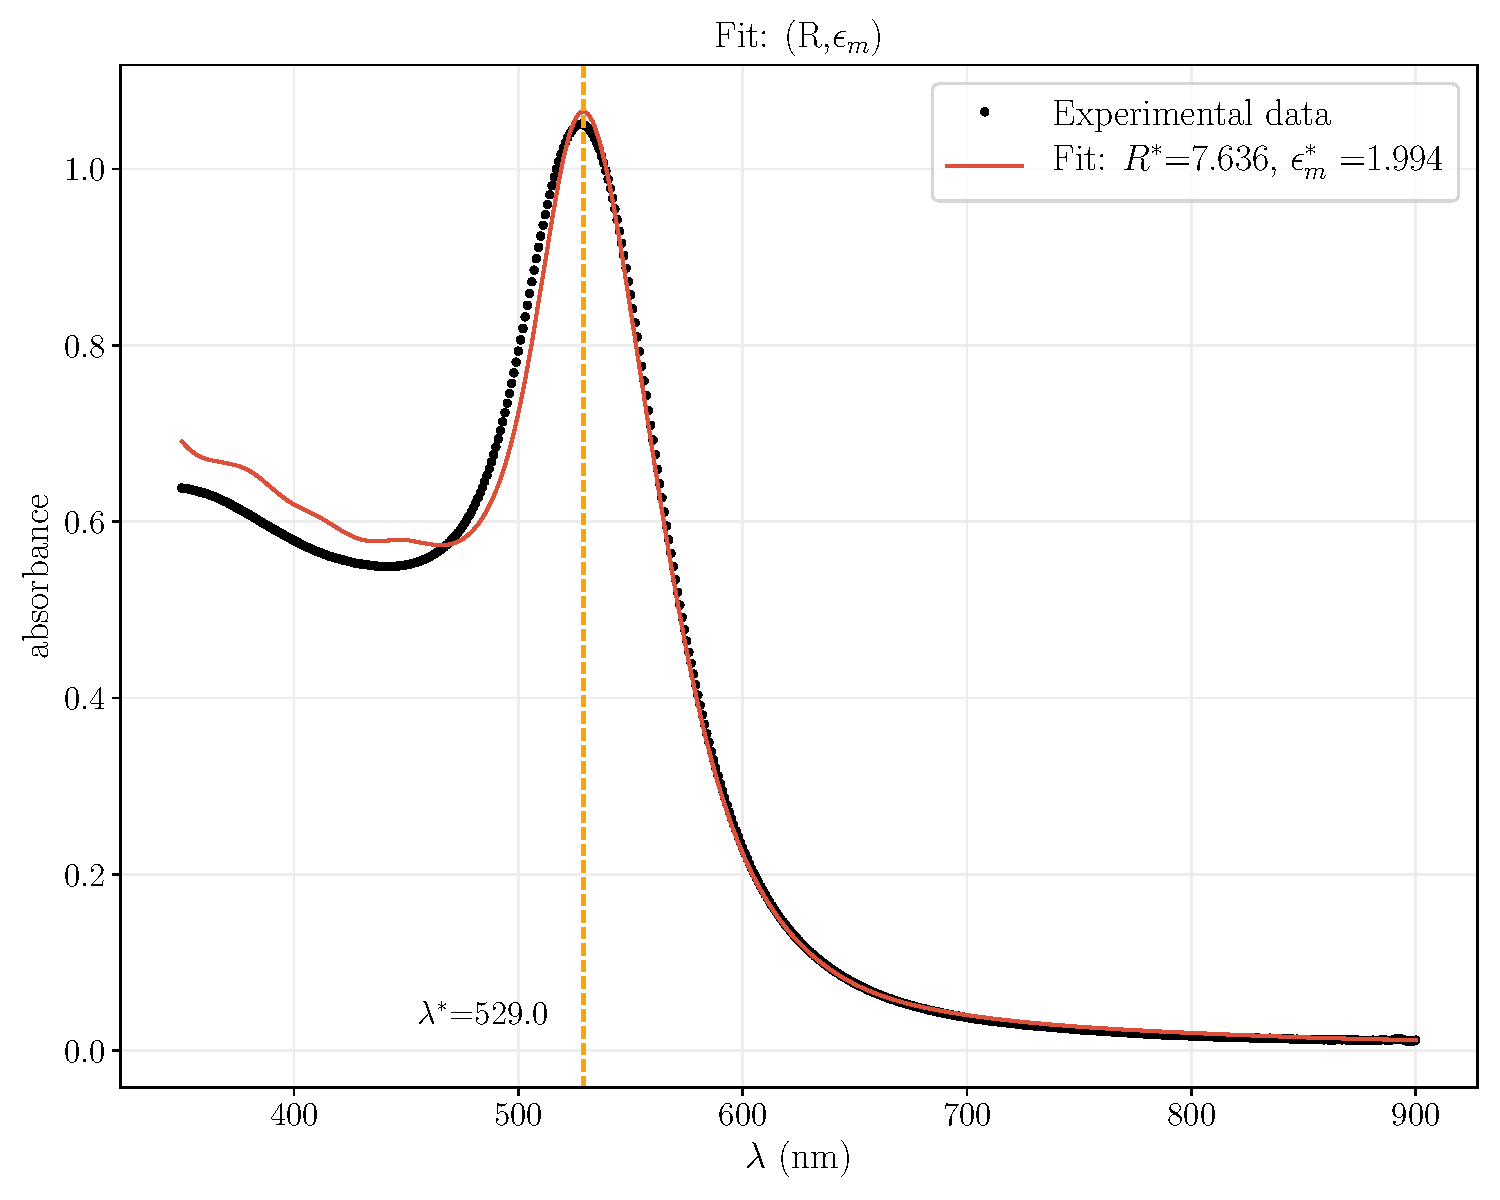
\includegraphics[width=0.49\textwidth]{images/os/2_fit_GANS.pdf}
    \\
    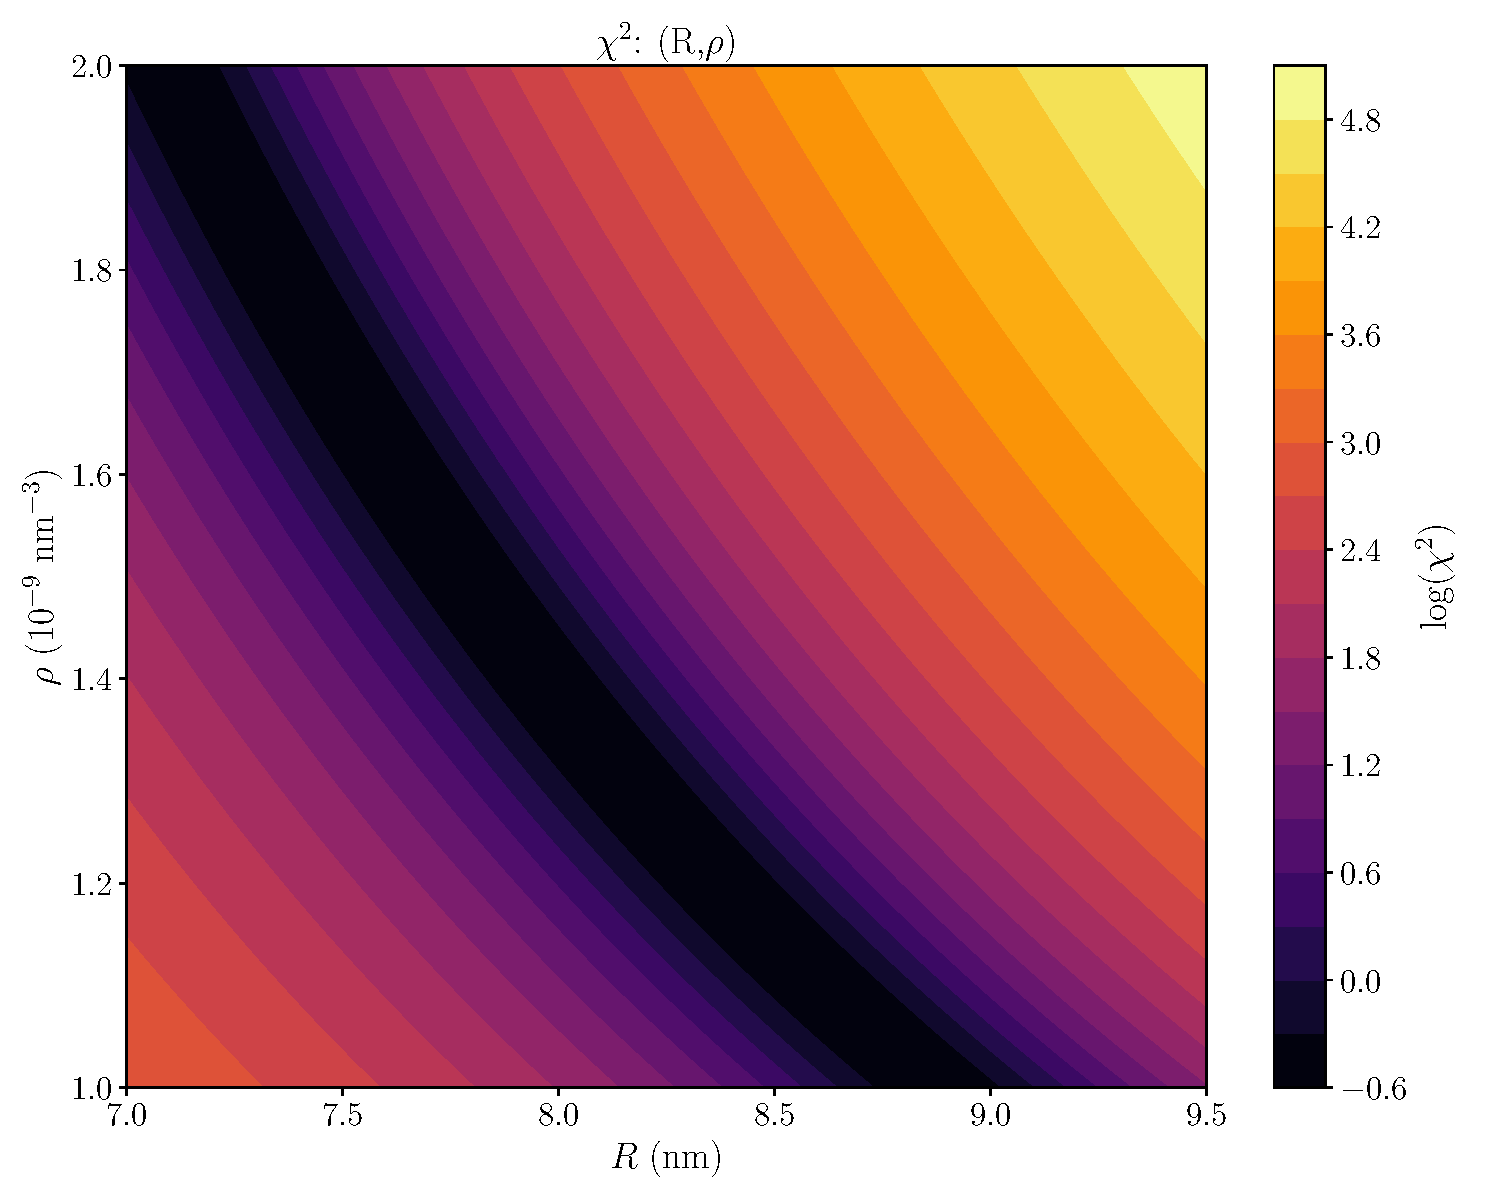
\includegraphics[width=0.49\textwidth]{images/os/1_chisquare_GANS.pdf}
   \hskip 1mm
   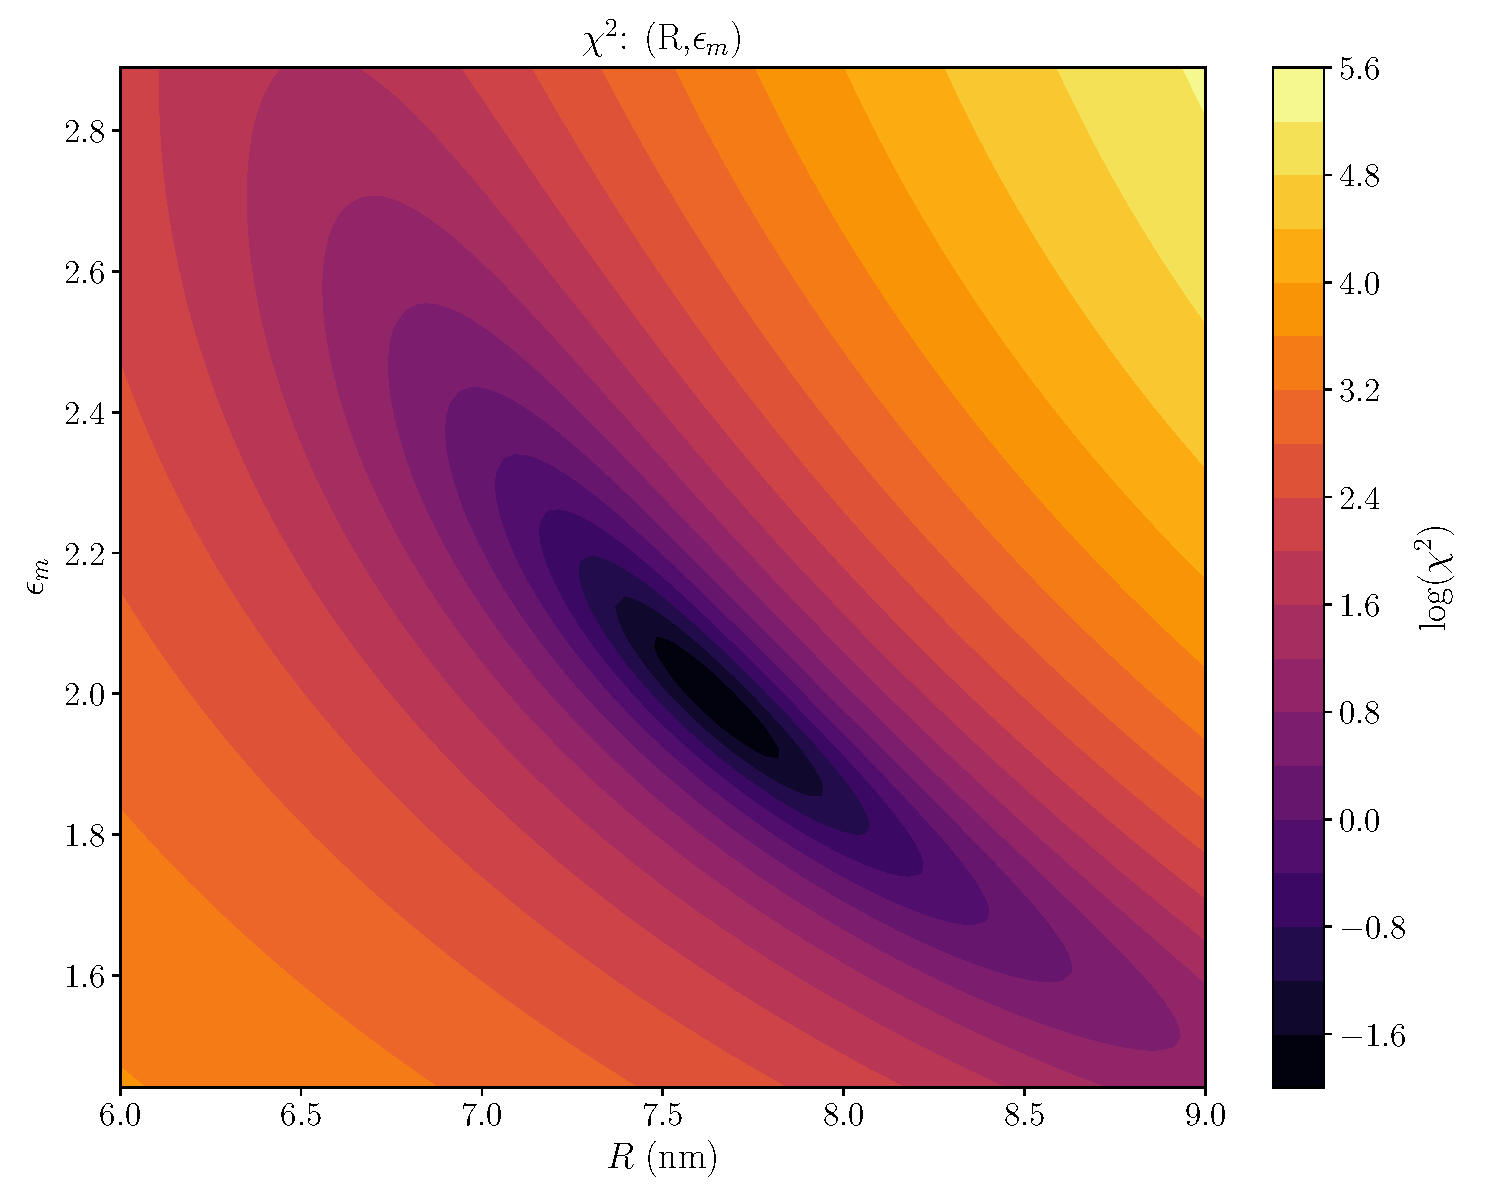
\includegraphics[width=0.49\textwidth]{images/os/2_chisquare_GANS.pdf}
    \caption{Gans theory. \textbf{Top}: on the left is represented the simulated spectrum obtained by varying the parameters $(R,\rho)$, while on the right the one obtained varying $(R,\epsilon_m)$. \textbf{Bottom}: on the left we have the $\chi^2$ map for $(R,\rho)$, on the right the one for $(R,\epsilon_m)$. }
    \label{fig:optical_results_GANS}
\end{figure*}

Anyway, in order to obtain a better agreement with SEM analysis, we repeat the optical analysis, taking into account the ellipsoidal shape of the nanoparticles. 
In fact, from SEM, we compute the average of the major and minor axis of the two dimensional representation of the particles, over all the datasets. The values obtained are:
\begin{equation*}
    a_1 = (23.951 \pm 0.009) \, \text{nm}, \quad a_2 = (20.154 \pm 0.009) \, \text{nm}
\end{equation*}
We suppose that the third axis is $a_3=a_2$. 

Then, we use the Gans theory which gives the representation of the extinction cross-section of an ensemble of elliposidal particles with spatial random orientation:
\begin{equation}
\sigma_{ext}^{\text{Gans}} = \frac{\omega}{3c} \epsilon_m^{3/2}V_{0} \sum^{3}_{j=1}{\frac{\epsilon_2/L_j^2}{[\epsilon_1 + \epsilon_m(1-L_j)/L_j]^2 + \epsilon_2^2}}
\end{equation}
The polarization coefficients $L_j$ are defined as 
\begin{subequations}
\begin{align}
  L_1 &= \frac{1-e^2}{e^2} \qty[\frac{1}{2e}\ln{\qty( \frac{1+e}{1-e})}-1] \\
  L_2 &= L_3 = \frac{1-L_1}{2} 
  \end{align}
\end{subequations}
where $e$ is the eccentricity.




%At first we simulate the spectrum for the couple $(R,\rho)$: we vary $R$ in the range $[7:9.5]$ nm and $\rho$ in $[1:2]\cdot 10^{-9} \text{nm}^{-3}$. Then, as far as the fit for $(R,\varepsilon_m)$ is concerned, we vary $\varepsilon_m$ in $[1.2:1.7]$. %

The simulated spectrum obtained, with the relative plot of $\chi^2$ stability, are illustrated in Fig.\ref{fig:optical_results_GANS}.
The best values for the three parameters $R$, $\rho$, $\epsilon_m$ are:
\begin{equation*}
    R^* = (8 \pm 1) \, \text{nm}, \quad \rho^* = (1 \pm 2) \cdot 10^{-9} \text{nm}^3 , \quad \epsilon_m^* = 2.0 \pm 0.1
\end{equation*}

We notice that, as expected, the radius computed by the Gans theory is more similar to the one of Scanning Electron Microscopy with respect to the radius computed assuming Mie theory. 
Also the fit quality is slightly improved: since ellipsoidal particle give a different position of the resonance for each length of the axis, the width of the peak can be better covered by the two resonances of our model.
Moreover, the value of the medium dielectric constant has slightly improved with respect to the expectations.
However, this is a retrospective analysis of the optical absorbance data, since we got the information on the particle shape from the SEM measurements. 


\section{Conclusion}
We characterized gold nanoparticles, synthetized by Turkevich method, with three different analysis: Optical Spectroscopy, X-rays and Scanning Electron Microscopy. 

In particular, from each method we obtained the average size of the nanoparticles. 
The result of SEM analysis is not compatible with the other two. However, since it is probably the most reliable method, we tried to explain why the other analysis may have lead to inaccurate results, and we tried to correct them as long as possible. 

Afterwards, from Optical Spectroscopy, we obtained also the order of magnitude of the numerical density of the particles $\rho$, in the colloidal solution,  and the dielectric constant of the medium $\epsilon_m$, which is not in agreement with what expected. 
From X-rays analysis, we verified the f.c.c. structure of gold nanoparticles by computing the lattice constant $a$ and by associating the corresponding Miller indexes to the peaks. 
Lastly, from Scanning Electron Microscopy, we found the size-distribution and the average aspect ratio of the nanoparticles.


\printbibliography

\vskip 0.4cm

\end{document}